\documentclass[11pt]{book}

% Shared HSC style packages (see ../HSC-Common/).
\makeatletter
\def\input@path{{../HSC-Common/styles/}{./}}
\makeatother
\newcommand{\HSCBookletHeaderTitle}{AUS Networks}

\usepackage{amsmath,amssymb,amsthm}
\usepackage{graphicx}
\usepackage{tikz}
\usetikzlibrary{positioning,arrows.meta,calc,shapes.geometric}
\usepackage{enumitem}
\usepackage{booktabs,tabularx,array}
\usepackage[most,skins]{tcolorbox}

% Shared DL101 booklet styles, loaded in dependency order.
\usepackage{dl101-colors}
\usepackage{dl101-hints}
\usepackage{dl101-boxes}
\usepackage{dl101-theorems}
\usepackage{dl101-hsc-problems}
\usepackage{dl101-diffeq-enrichment}
\usepackage{dl101-layout}

% Links without visible rectangles (TOC and cross-references remain clickable).
\usepackage[hidelinks,hypertexnames=false]{hyperref}
\hypersetup{hidelinks}

\setlength{\parindent}{0pt}
\setlength{\parskip}{0.55em}
\setlist[enumerate]{leftmargin=*,itemsep=0.3em}
\setlist[itemize]{leftmargin=*,itemsep=0.25em}
\newcommand{\Core}{\textsf{[Core]}}
\newcommand{\Challenge}{\textsf{[Challenge]}}
\newcommand{\Investigation}{\textsf{[Investigation]}}
\newcommand{\Coding}{\textsf{[Optional coding]}}
\newcommand{\Enrichment}{\textsf{[Enrichment]}}
\newcommand{\Uni}{\textsf{[Uni-level]}}
\newcommand{\WarningSign}{\tikz[baseline=-0.6ex]\node[draw,regular polygon,regular polygon sides=3,inner sep=0pt,minimum size=1.1em,line width=0.35pt] {!};}
\newcommand{\V}{V}
\newcommand{\E}{E}
\newcommand{\degG}{\operatorname{deg}}
\newcommand{\dist}{\operatorname{dist}}
\newcommand{\chiG}{\chi}
\newcommand{\set}[1]{\left\{#1\right\}}
\title{AUS-Graphs: An Introduction to Graph Theory for Extension and Specialist Students}
\author{Vu Hung Nguyen}
\date{2026}

\begin{document}

% Unnumbered matte cover.
\begin{titlepage}
\newgeometry{margin=0pt}
\thispagestyle{empty}
\begin{tikzpicture}[remember picture,overlay]
  \node[anchor=south west,inner sep=0pt] at (current page.south west) {%
    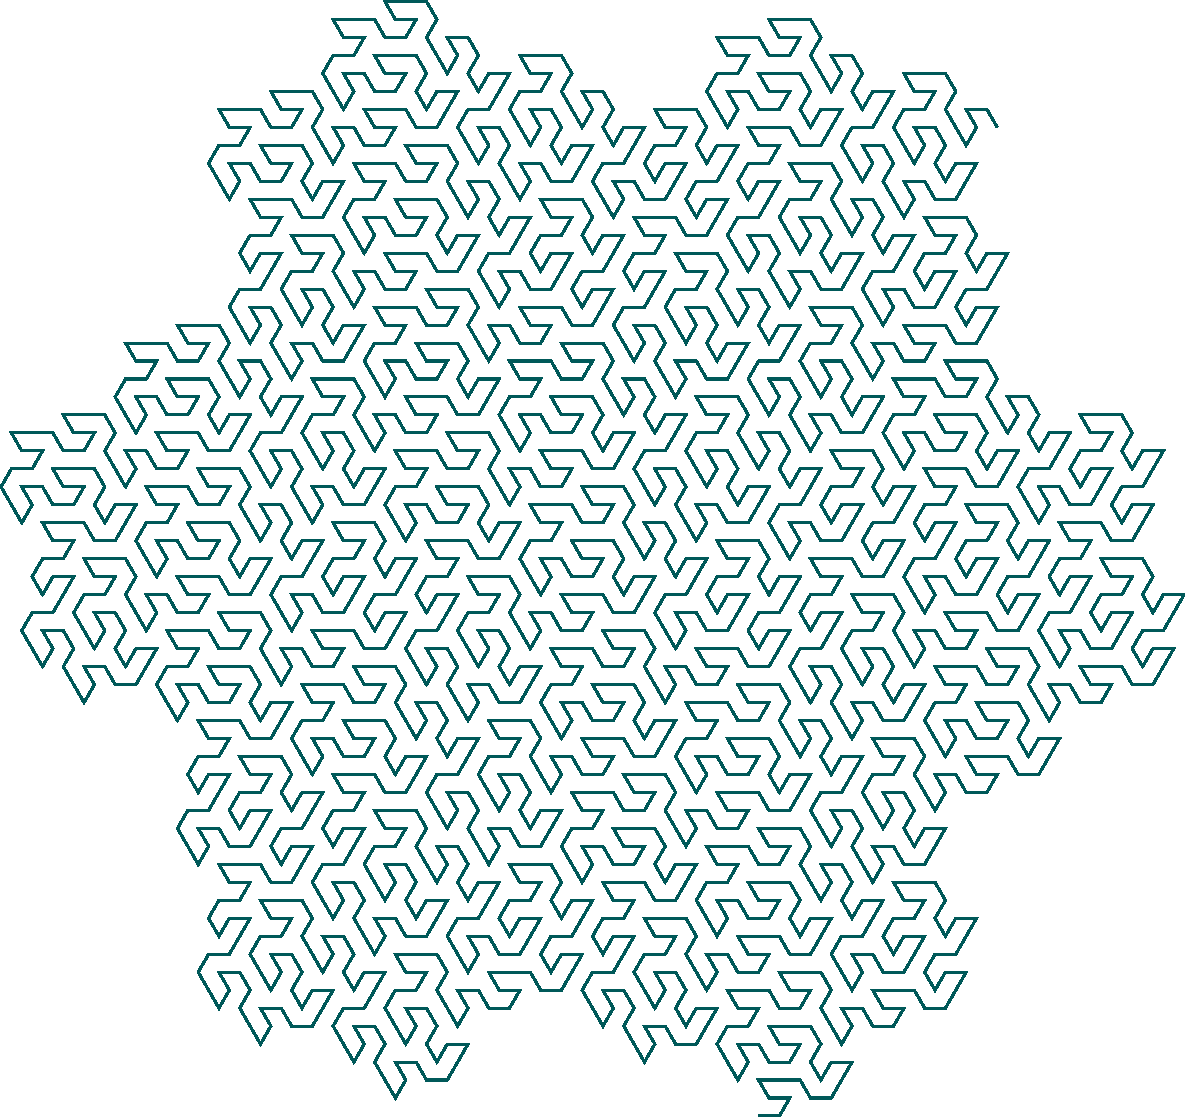
\includegraphics[width=\paperwidth,height=\paperheight]{assets/matte-generator.pdf}%
  };
  \fill[black,opacity=0.3]
    (current page.south west) rectangle (current page.north east);
  \node[
    align=center,
    text=white,
    fill=black,
    fill opacity=0.45,
    text opacity=1,
    rounded corners=2pt,
    inner xsep=10pt,
    inner ysep=8pt
  ] at (current page.center) {%
    \begin{minipage}{0.86\paperwidth}
      \centering
      \HSCMatteTitleText
        {Extension and Specialist Mathematics}
        {AUS-Networks\\[0.2cm]\Large An Introduction to Graph Theory}
        {Vu Hung Nguyen}
    \end{minipage}%
  };
\end{tikzpicture}
\null
\restoregeometry
\end{titlepage}

% Numbered front matter: QR codes (1), quote (2), warning (3), contents (4).
\pagenumbering{arabic}
\setcounter{page}{1}

\thispagestyle{empty}
% Shared QR code page content (page 2): GitHub repo + Vu’s Maths Hub, side by side.
\vspace*{\fill}
\begin{center}
\begin{minipage}[c]{0.4\textwidth}
  \centering
  
\includegraphics[width=0.9\linewidth]{assets/qrcode.png}\\[0.4cm]
  {\small\itshape Download PDF and resources:}\\[0.15cm]
  {\footnotesize\url{https://github.com/vuhung16au/math-olympiad-ml}}
\end{minipage}%
\hfill
\begin{minipage}[c]{0.4\textwidth}
  \centering
  
\includegraphics[width=0.9\linewidth]{assets/qrcode-vumaths.png}\\[0.4cm]
  {\small\itshape Read online at Vu's Maths Hub:}\\[0.15cm]
  {\footnotesize\url{https://vumaths.com/}}
\end{minipage}
\end{center}
\vspace*{\fill}

\begingroup\small\noindent
This work is licensed under CC BY-NC 4.0 (Attribution-Non-Commercial), see the LICENSE file on the GitHub page for more information.
\par\endgroup

\clearpage
\thispagestyle{empty}
\vspace*{\fill}
\begin{center}
\itshape
``Truth is ever to be found in the simplicity, and not in the multiplicity and confusion of things.''

\vspace{1em}
\normalfont Sir Isaac Newton
\end{center}
\vspace*{\fill}

\clearpage
\thispagestyle{empty}
\vspace*{\fill}
\begin{center}
\begin{tcolorbox}[
  width=0.88\textwidth,
  colback=black!5,
  colframe=black,
  boxrule=0.8pt,
  arc=2pt,
  left=12pt,
  right=12pt,
  top=12pt,
  bottom=12pt
]
\centering
\textbf{\Large \WarningSign\ ENRICHMENT ONLY --- OSS (OUT OF SYLLABUS)}

\vspace{0.8em}

\normalsize Do not use this booklet as exam preparation. It has no NESA HSC weighting and should never replace study of your official syllabus, school notes, or past examination papers.
\end{tcolorbox}
\end{center}
\vspace*{\fill}

\clearpage
\tableofcontents
\clearpage

\chapter*{Guide to AUS-Graphs}
\addcontentsline{toc}{chapter}{Guide to AUS-Graphs}
\section*{Introduction}

\subsection*{About This Booklet}
AUS-Graphs is an introduction to graph theory: the mathematics of networks and connections. It develops the subject from its basic language to structural results, colouring, optimisation and algorithms. The current edition is theory-focused, with examples and a substantial set of exercises; it is not an examination-preparation text.

\subsection*{Target Audience}
This booklet is for curious senior mathematics students in Australia, especially those studying extension or specialist mathematics. It is also suitable for independent readers who enjoy mathematical reasoning and want to explore a subject linking proof, counting, geometry, computing and real-world models.

\subsection*{Why This Book?}
Graph and network ideas appear across senior mathematics courses in New South Wales, Victoria and Queensland, but their scope, emphasis and assumed background are not identical. This booklet gives students from all three states a shared starting point and develops the ideas consistently, without assuming that a topic has already been taught in a particular course. It is also intended to help students build the reasoning and problem-solving skills used in olympiad-style mathematics competitions, and to prepare interested readers for further study, especially discrete mathematics.

\subsection*{A Foundation for Further Study}
The ideas in this booklet build foundations in graph theory and discrete mathematics, and offer a first look at concepts that also appear in the foundations of computer science. These subjects feature in higher studies, including undergraduate mathematics and applied mathematics. This booklet is a starting point for that study, not a substitute for university-level courses.

\subsection*{How to Use This Booklet}
The main chapters build ideas in sequence, from modelling situations as graphs to proving structural results and applying algorithms. Sections marked \Core{} form the main path; the five central proved theorems are also marked \Core{}. Their proofs are given in the text. \Challenge{} sections go further, while \Investigation{} prompts invite exploration with more than one possible outcome. \Enrichment{} sections offer optional extensions that remain accessible with the booklet's background. \Uni{} sections preview ideas usually developed in undergraduate mathematics and may use unfamiliar concepts. \Coding{} activities are optional; pseudocode or a spreadsheet can be used instead of a programming language. Every numbered exercise has an answer or brief solution in the back matter; challenging exercises also have hints, while open-ended investigations have sample approaches.

\subsection*{Knowledge Needed}
Familiarity with algebra, basic counting and the idea of mathematical proof is helpful, but no particular state course or prior graph theory is assumed. The booklet introduces the definitions and methods it uses. Here is a quick guide to some shared language and notation:
\begin{itemize}
\item \textbf{Numbers and algebra:} A letter such as $n$ or $k$ stands for a number. For example, $2k$ is even, and $n-1$ means one less than $n$.
\item \textbf{Sets and graph notation:} A graph is written $G=(V,E)$: $V$ is its set of vertices (the objects) and $E$ is its set of edges (the connections). In a graph with vertices labelled $v_1,v_2,\ldots,v_n$, the subscripts are labels, not powers.
\item \textbf{Graph drawings:} Vertices are shown as solid dots when their names are not needed. When a discussion depends on identifying particular vertices, they are shown as labelled circles.
\item \textbf{Counting pairs:} The notation $\binom{n}{2}$ counts the ways to choose two objects from $n$ when order does not matter. For example, $\binom{7}{2}=21$.
\item \textbf{Proof:} A proof explains why a statement must be true. To disprove a claim that is supposed to hold in every case, one counterexample is enough.
\item \textbf{Matrices:} A matrix is a rectangular array of numbers. Its size is given as rows $\times$ columns; $A_{ij}$ means the entry in row $i$, column $j$. In the example below, the 1s record which pairs of vertices are joined. No matrix knowledge is assumed: the later bridge module explains how to read and use these arrays.
\end{itemize}

\begin{figure}[htbp]
\centering
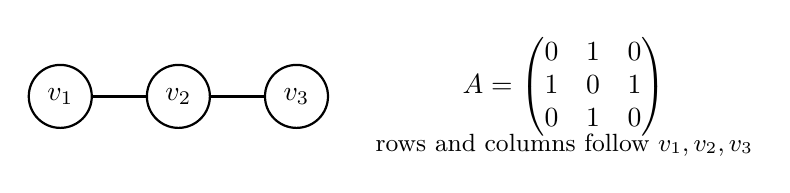
\begin{tikzpicture}[thick,every node/.style={circle,draw,fill=white,minimum size=8mm}]
\node (v1) at (0,0) {$v_1$};
\node (v2) at (1.5,0) {$v_2$};
\node (v3) at (3,0) {$v_3$};
\draw (v1)--(v2)--(v3);
\node[draw=none,rectangle,align=center] at (6.4,0) {$A=\begin{pmatrix}0&1&0\\1&0&1\\0&1&0\end{pmatrix}$\\[-0.2em]\small rows and columns follow $v_1,v_2,v_3$};
\end{tikzpicture}
\caption{The graph and its adjacency matrix: for example, $A_{12}=1$ because $v_1$ and $v_2$ are joined, while $A_{13}=0$ because they are not.}
\end{figure}

The chapters also explain the graph-specific terms as they arise. Readers who already know matrices may skim the bridge module, while others can use it as a first introduction to the matrix ideas needed here.

\subsection*{What You Will Learn}
You will learn to model connections with graphs; reason about degrees, paths, cycles, trees and planarity; develop and communicate proofs; and use colouring and algorithms to study network problems. The applied appendix provides a bridge to selected network methods used in senior mathematics courses.

\chapter*{A quick diagnostic}
Try these without looking anything up. The point is to identify useful skills, not to earn a score.
\begin{enumerate}
\item How many different pairs can be selected from 7 people?
\item Give an example that disproves the claim: ``If a number is divisible by 4, then it is odd.''
\item Explain why the sum of two even integers is even.
\item A process has three stages, each of which must finish before the next begins. Draw a diagram showing the order.
\item If a square matrix has a 1 in position $(i,j)$, what information might that entry record in a network?
\end{enumerate}
Useful responses: $\binom72=21$; any multiple of 4 is a counterexample; write the integers as $2a$ and $2b$; draw a chain of three labelled stages; and an entry can record whether there is a connection from object $i$ to object $j$. If some items are unfamiliar, the chapters build these ideas from the ground up.
\mainmatter
\part{Problems that lead to graphs}
\chapter{Problems that lead to graphs}
\section*{A map with too many details}
Imagine planning a trip between towns. A literal map contains buildings, terrain, road widths and labels, most of which do not matter if the only question is which towns are connected by roads. A mathematical model keeps the relevant information and discards the rest. Graphs are models of connections.

One question to keep in mind: \emph{What's the fastest way to get from Town Hall to the Blue Mountains?}

In 1736 Leonhard Euler studied the bridges of Königsberg. The question was whether a walk could cross each bridge exactly once. The key insight was to replace each land mass by a point and each bridge by a line. The shape of the map did not matter; the incidence pattern did.

\begin{definition}
A (finite, undirected) \emph{graph} is a triple $G=(V,E,\psi)$, where $V$ is a nonempty finite set of vertices, $E$ is a finite set of edges disjoint from $V$, and $\psi$ assigns to each edge an unordered pair of vertices in $V$ (its endpoints). The endpoints may be equal, giving a \emph{loop}, and distinct edges may have the same endpoints, giving \emph{parallel edges}.
\end{definition}

Unless stated otherwise, this booklet studies \emph{simple graphs}: graphs with no loops or parallel edges. In this case, each edge corresponds to a pair of distinct vertices, so we can write $G=(V,E)$, with $E$ a set of such pairs.

Two distinct vertices are \emph{adjacent} if an edge joins them. An edge is \emph{incident} with a vertex if that vertex is one of its endpoints.

\begin{figure}[h]
\centering
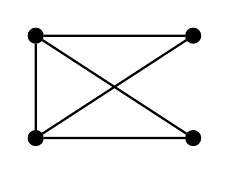
\begin{tikzpicture}[every node/.style={circle,draw=black,fill=black,inner sep=0pt,minimum size=5pt},thick]
\node (A) at (0,1.3) {}; \node (B) at (2,1.3) {}; \node (C) at (0,0) {}; \node (D) at (2,0) {};
\draw (A)--(B) (A)--(C) (A)--(D) (B)--(C) (C)--(D);
\end{tikzpicture}
\caption{A simple graph with four vertices and five edges.}
\end{figure}

The vertices might represent people, towns, tasks or websites. An edge records the relation of interest: friendship, a road, a prerequisite or a hyperlink. A good model makes the question precise. If roads have travel times, use a \emph{weighted graph}; if a connection has a direction, use a \emph{directed graph}; if two towns have several distinct roads between them, use a \emph{multigraph}.

To model the opening question, first choose a travel mode and a destination in the Blue Mountains. For a driving model, let vertices represent road junctions and edges represent road segments; use directed edges for one-way roads. Give each edge an estimated travel-time weight, perhaps for a specified departure time. A journey is then represented by a path, and its total travel time is the sum of its edge weights. The fastest journey is a path of minimum total weight, which need not use the fewest roads or cover the shortest distance.

A different question is how to connect several electricity-network hubs at the lowest total construction cost. Represent the hubs by vertices, possible links by edges, and estimated costs by weights. If the only requirement is to connect every hub without redundant links, the model asks for a minimum spanning tree. This is a deliberately simplified teaching model: real electricity-network design also has to account for reliability, capacity, demand and engineering constraints, among others.

\section{From situation to graph}
A modelling checklist:
\begin{enumerate}
\item Decide what the vertices represent.
\item Decide what an edge means, including whether direction or repetition matters.
\item Add weights or labels only when the question needs them.
\item Check whether the model preserves the feature you want to study.
\end{enumerate}
For a timetable conflict graph, each vertex can represent a class and an edge can join two classes that share students. A proper colouring then assigns times so that conflicting classes get different times.

\section{When are two drawings the same graph?}
The same graph can be drawn with vertices in different places and edges bent or straight. Two graphs are \emph{isomorphic} if there is a bijection between their vertices such that two vertices are adjacent exactly when their corresponding vertices are adjacent. In other words, the names and layout may change, but the connection pattern does not.

\begin{example}
A triangle drawn as a triangle and the same three vertices drawn at the corners of a curved shape are isomorphic: every pair is joined. By contrast, a three-vertex path is not isomorphic to a triangle, because the path has two edges and the triangle has three.
\end{example}

To show two graphs are not isomorphic, find a property preserved by isomorphism that differs: number of vertices, number of edges, degrees, number of components, or cycle lengths. Matching these properties does not by itself prove isomorphism; a valid vertex correspondence must preserve every edge.

\section*{Exercises}
\begin{enumerate}
\item Draw a graph for five people where an edge means ``has exchanged a book with''. What information is lost if you draw only whether an exchange has ever happened?
\item A one-way social-media follow relation is modelled by a graph. What kind? How might you model how many messages were exchanged?
\item Can two non-isomorphic graphs have the same number of vertices and edges? Draw an example on four vertices.
\item A school wants to schedule exams with no student required to sit two exams at once. Describe a graph model and explain what a colouring represents.
\end{enumerate}

\chapter{Degrees, counting and proof}
\section*{An odd fact about handshakes}
If everyone at a gathering shakes hands with some of the others, can exactly one person have shaken hands with an odd number of people? The answer is no, and the reason is one of the simplest and most useful graph proofs.

\begin{definition}
The \emph{degree} $\degG(v)$ of a vertex $v$ is the number of edges incident with it, counting parallel edges separately and each loop twice. A vertex of degree 0 is isolated. A vertex adjacent to every other vertex is universal. A vertex is \emph{odd} if its degree is odd, and \emph{even} otherwise.
\end{definition}

\begin{figure}[htbp]
\centering
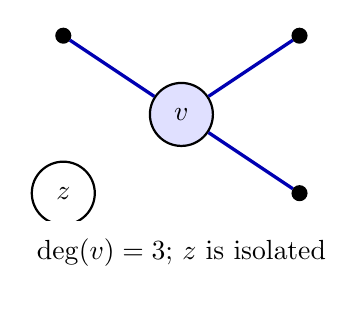
\begin{tikzpicture}[thick,every node/.style={circle,draw,fill=white,minimum size=8mm}]
\node[fill=blue!12] (v) at (0,0) {$v$};
\node[circle,draw=black,fill=black,inner sep=0pt,minimum size=5pt] (a) at (-1.5,1) {};
\node[circle,draw=black,fill=black,inner sep=0pt,minimum size=5pt] (b) at (1.5,1) {};
\node[circle,draw=black,fill=black,inner sep=0pt,minimum size=5pt] (c) at (1.5,-1) {};
\node (z) at (-1.5,-1) {$z$};
\draw[blue!70!black,line width=1.2pt] (v)--(a) (v)--(b) (v)--(c);
\node[draw=none,rectangle] at (0,-1.75) {$\degG(v)=3$; $z$ is isolated};
\end{tikzpicture}
\caption{The degree counts the edges incident with a vertex.}
\end{figure}

\begin{theorem}[\Core{} Handshaking lemma]
For any finite undirected graph, $\sum_{v\in V}\degG(v)=2|E|$.
\end{theorem}
\begin{figure}[htbp]
\centering
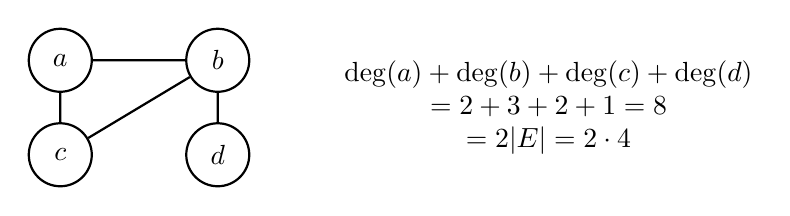
\begin{tikzpicture}[thick,every node/.style={circle,draw,fill=white,minimum size=8mm}]
\node (a) at (0,1.2) {$a$}; \node (b) at (2,1.2) {$b$};
\node (c) at (0,0) {$c$}; \node (d) at (2,0) {$d$};
\draw (a)--(b) (a)--(c) (b)--(c) (b)--(d);
\node[draw=none,rectangle,align=center] at (6.2,0.6) {$\degG(a)+\degG(b)+\degG(c)+\degG(d)$\\$=2+3+2+1=8$\\$=2|E|=2\cdot4$};
\end{tikzpicture}
\caption{Each edge contributes one incidence at each of its two endpoints.}
\end{figure}
\begin{proof}
Count endpoint-incidences, where each incidence pairs an edge with one of its two endpoint occurrences. Each edge contributes two incidences, including a loop, whose two incidences are with the same vertex. Counting instead by vertex, vertex $v$ contributes $\degG(v)$ incidences. These are two counts of the same set, hence the equality.
\end{proof}

\begin{corollary}
Every finite undirected graph has an even number of odd-degree vertices.
\end{corollary}
\begin{figure}[htbp]
\centering
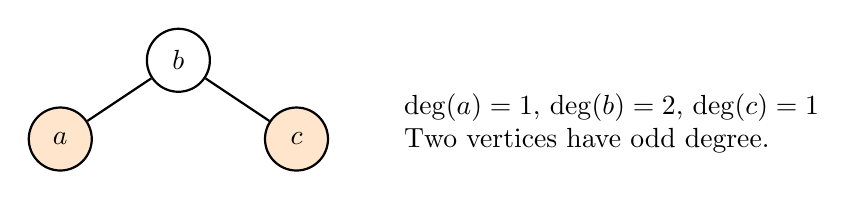
\begin{tikzpicture}[thick,every node/.style={circle,draw,fill=white,minimum size=8mm}]
\node[fill=orange!20] (a) at (0,0) {$a$};
\node[fill=white] (b) at (1.5,1) {$b$};
\node[fill=orange!20] (c) at (3,0) {$c$};
\draw (a)--(b)--(c);
\node[draw=none,rectangle,align=left] at (7,0.2) {$\degG(a)=1$, $\degG(b)=2$, $\degG(c)=1$\\Two vertices have odd degree.};
\end{tikzpicture}
\caption{Odd-degree vertices occur in pairs (here, the two orange endpoints).}
\end{figure}
\begin{proof}
The sum of all degrees is even by the handshaking lemma. A sum of integers is even precisely when it contains an even number of odd summands. Therefore the number of odd-degree vertices is even.
\end{proof}

\begin{definition}
The complete graph $K_n$ has $n$ vertices and an edge between every pair of distinct vertices. A graph is \emph{bipartite} if its vertices can be divided into two sets so every edge joins one set to the other. The cycle graph $C_n$ is a single cycle on $n$ vertices.
\end{definition}

\begin{figure}[htbp]
\centering
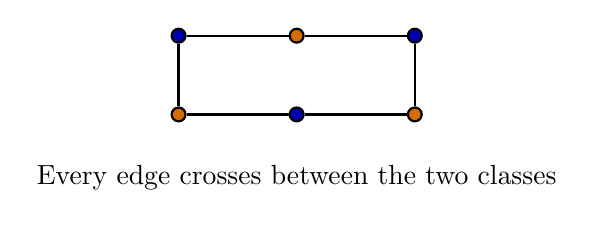
\begin{tikzpicture}[thick,vertex/.style={circle,draw=black,fill=black,inner sep=0pt,minimum size=5pt}]
\node[vertex,fill=blue!70!black] (a) at (0,1) {};
\node[vertex,fill=orange!85!black] (b) at (1.5,1) {};
\node[vertex,fill=blue!70!black] (c) at (3,1) {};
\node[vertex,fill=orange!85!black] (d) at (3,0) {};
\node[vertex,fill=blue!70!black] (e) at (1.5,0) {};
\node[vertex,fill=orange!85!black] (f) at (0,0) {};
\draw (a)--(b)--(c)--(d)--(e)--(f)--(a);
\node[draw=none,rectangle,fill=white] at (1.5,-0.8) {Every edge crosses between the two classes};
\end{tikzpicture}
\caption{The even cycle $C_6$ is bipartite: adjacent vertices have opposite colours.}
\end{figure}

In $K_n$, each vertex has degree $n-1$. Thus $2|E|=n(n-1)$ and $|E|=\binom n2$. The complete bipartite graph $K_{r,s}$ has $r+s$ vertices and $rs$ edges.

\begin{example}
A graph has degree sequence $3,3,2,2,2$. The sum is 12, so it has 6 edges. A proposed degree sequence $3,3,3,1$ cannot describe a graph: it has three odd entries, contradicting the corollary.
\end{example}

A counterexample is often the shortest way to disprove a universal claim. For instance, ``every graph with an even number of vertices has an even number of edges'' fails for a triangle together with an isolated vertex: four vertices, three edges.

\begin{theorem}[\Challenge{} A degree-sum test for connectedness]
Let $G$ be a finite simple graph on $n\geq 1$ vertices. If every pair of nonadjacent vertices $u,v$ satisfies $\degG(u)+\degG(v)\geq n-1$, then $G$ is connected; in fact, any two vertices are at distance at most 2.
\end{theorem}
\begin{proof}
Take any two distinct vertices $u,v$. If they are adjacent, they are joined by a path of length 1. Otherwise, let $N(u)$ and $N(v)$ be their sets of neighbours; both lie among the other $n-2$ vertices. Since
\[
|N(u)|+|N(v)|=\degG(u)+\degG(v)\geq n-1>n-2,
\]
the two neighbour sets must overlap. A common neighbour gives a path of length 2 from $u$ to $v$. Thus every pair is joined by a path of length at most 2.
\end{proof}

\Enrichment{} \textbf{Havel--Hakimi reduction.} To test a nonincreasing sequence of nonnegative integers, remove its largest term $d$ and subtract 1 from the next $d$ terms, then reorder. The Havel--Hakimi theorem says the original sequence is graphical exactly when this process reaches the all-zero sequence; a negative term or too few remaining terms makes it non-graphical.

\section*{Exercises}
\begin{enumerate}
\item Prove that in any simple graph on $n$ vertices, every degree is at most $n-1$.
\item How many edges are in $K_{12}$ and in $K_{4,7}$?
\item A graph has 9 edges. Can all its vertices have degree 3? If so, how many vertices must it have?
\item Disprove: ``If a graph has an even number of edges, then every vertex has even degree.''
\item \Challenge{} The Petersen graph has 10 vertices, each of degree 3. Use the handshaking lemma to find its number of edges.
\item \Enrichment{} Apply the Havel--Hakimi reduction to the sequence $3,3,2,2,2$. (a) Remove the largest term and reduce the next terms as prescribed; reorder the result. (b) Repeat until you reach zeros or detect that the sequence is not graphical. (c) Starting from the last reduction, reverse your steps to construct a graph with the original degree sequence, then check its degrees. (d) Try the same test on $3,3,1,1$. At which step does it fail?
\end{enumerate}

\chapter{Paths and connectedness}
\section*{Can every place be reached?}
When a network has no route between some pair of locations, it breaks into separate regions. To reason accurately about routes, distinguish a walk, which may repeat, from a path, which does not repeat vertices.

\begin{definition}
A \emph{walk} is a finite sequence of vertices with consecutive vertices adjacent. A \emph{trail} is a walk that does not repeat edges. A \emph{path} is a walk that does not repeat vertices. A \emph{cycle} is a closed walk of length at least 3 in which no vertex is repeated except that the starting and ending vertices are the same. A graph is \emph{connected} if every pair of vertices is joined by a path; otherwise its maximal connected pieces are its \emph{components}.
\end{definition}

\begin{figure}[htbp]
\centering
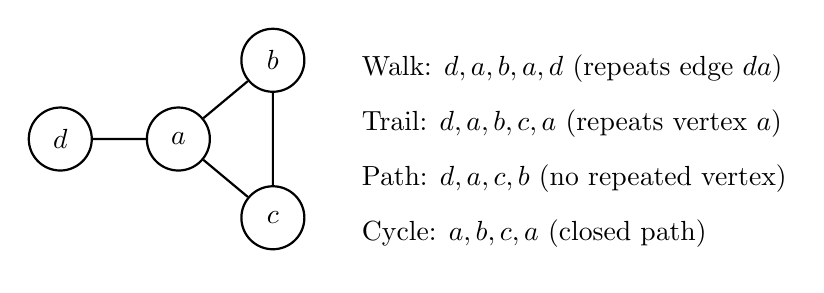
\begin{tikzpicture}[thick,every node/.style={circle,draw,fill=white,minimum size=8mm}]
\node (a) at (0,0) {$a$}; \node (b) at (1.2,1) {$b$};
\node (c) at (1.2,-1) {$c$}; \node (d) at (-1.5,0) {$d$};
\draw (a)--(b)--(c)--(a) (a)--(d);
\node[draw=none,rectangle,anchor=west] at (2.2,0.9) {Walk: $d,a,b,a,d$ (repeats edge $da$)};
\node[draw=none,rectangle,anchor=west] at (2.2,0.2) {Trail: $d,a,b,c,a$ (repeats vertex $a$)};
\node[draw=none,rectangle,anchor=west] at (2.2,-0.5) {Path: $d,a,c,b$ (no repeated vertex)};
\node[draw=none,rectangle,anchor=west] at (2.2,-1.2) {Cycle: $a,b,c,a$ (closed path)};
\end{tikzpicture}
\caption{Walks may repeat edges; trails may repeat vertices; paths repeat neither.}
\end{figure}

\begin{theorem}[\Core{} A walk contains a path]
If there is a $u$--$v$ walk in a graph, then there is a $u$--$v$ path.
\end{theorem}
\begin{proof}
Choose a $u$--$v$ walk of minimum length. If a vertex occurs twice, remove the part of the walk between two of its occurrences. The result is a shorter $u$--$v$ walk, contradicting minimality. Thus no vertex repeats, so the walk is a path.
\end{proof}
This simple fact lets us replace a route that may repeat vertices by one that does not.

\begin{theorem}[\Core{} Bipartite graphs and odd cycles]
A graph is bipartite if and only if it contains no odd cycle.
\end{theorem}
\begin{figure}[htbp]
\centering
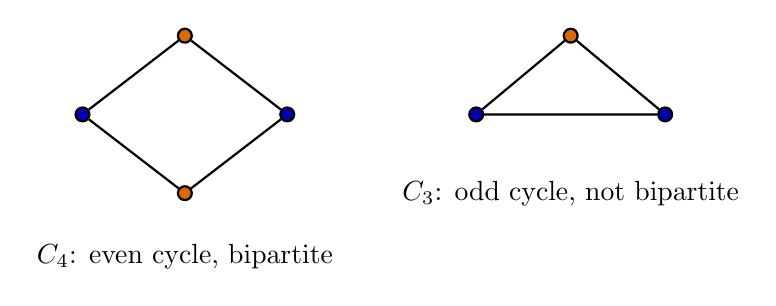
\begin{tikzpicture}[thick,vertex/.style={circle,draw=black,fill=black,inner sep=0pt,minimum size=5pt}]
\node[vertex,fill=blue!70!black] (a) at (0,0) {};
\node[vertex,fill=orange!85!black] (b) at (1.3,1) {};
\node[vertex,fill=blue!70!black] (c) at (2.6,0) {};
\node[vertex,fill=orange!85!black] (d) at (1.3,-1) {};
\draw (a)--(b)--(c)--(d)--(a);
\node[draw=none,rectangle,fill=white] at (1.3,-1.8) {$C_4$: even cycle, bipartite};
\node[vertex,fill=blue!70!black] (p) at (5,0) {};
\node[vertex,fill=orange!85!black] (q) at (6.2,1) {};
\node[vertex,fill=blue!70!black] (r) at (7.4,0) {};
\draw (p)--(q)--(r)--(p);
\node[draw=none,rectangle,fill=white] at (6.2,-1) {$C_3$: odd cycle, not bipartite};
\end{tikzpicture}
\caption{Alternating two classes succeeds around an even cycle but fails around an odd one.}
\end{figure}
\begin{proof}
If a graph is bipartite, a walk alternates between the two vertex classes at each step. Returning to the starting class therefore takes an even number of steps, so every cycle has even length.

Conversely, suppose the graph has no odd cycle. Work within one component and choose a starting vertex $r$. Put each vertex in one of two classes according to whether its shortest-path distance from $r$ is even or odd. If an edge joined two vertices at the same parity, shortest paths from $r$ to those endpoints together with the edge would contain an odd closed walk. Every odd closed walk contains an odd cycle: if any vertex appears at two occurrences beyond the required equality of the first and last vertices, split the walk at those occurrences. The two shorter closed walks have lengths summing to the original odd length, so one is odd. Keep that shorter odd closed walk and repeat; because the lengths decrease, this process ends with an odd cycle. This contradicts the assumption. So each edge joins opposite classes. Repeat for each component.
\end{proof}

\section*{Breadth-first search: exploring by layers}
Breadth-first search (BFS) explores a graph from a chosen starting vertex in layers: first the start, then vertices one edge away, then vertices two edges away, and so on. In an unweighted graph, the first path found to a vertex uses the fewest edges.

To find a path from a source $s$ to a target $t$:
\begin{enumerate}
\item Put $s$ in a first-in, first-out queue, mark it as discovered, and record that it has no predecessor.
\item Remove the vertex $u$ at the front of the queue and inspect each of its neighbours.
\item For every neighbour $v$ not yet discovered, mark $v$ as discovered, record $u$ as its predecessor, and add $v$ to the back of the queue.
\item Continue until $t$ is discovered or the queue is empty. If $t$ is discovered, follow the predecessor records back to $s$ to recover a shortest path in number of edges.
\end{enumerate}

For the Town Hall journey, BFS would find a route using the fewest road segments if each road segment counts as one edge. It does not necessarily find the fastest route when segments have different travel times: a route with more quick segments can take less time than one with fewer slow segments. The Dijkstra section later in the book explains how to handle non-negative travel-time weights. Depth-first search (DFS), by contrast, follows one branch as far as possible before backtracking. BFS and DFS can both be implemented with a queue or stack and a set of discovered vertices.

\section*{Exercises}
\begin{enumerate}
\item In a square with one diagonal, list a walk of length 4 that is not a trail, and a trail that is not a path.
\item Is a 7-cycle bipartite? Justify your answer. What about a 10-cycle?
\item Draw a disconnected graph with exactly three components and list their sizes.
\item \Coding{} Starting at a chosen vertex, perform BFS on a graph of your own design and record the order vertices are first visited. Compare with DFS.
\end{enumerate}

\chapter*{Bridge module: Matrices and graphs}
\addcontentsline{toc}{chapter}{Bridge module: Matrices and graphs}
A matrix is a rectangular array of numbers. For a graph with labelled vertices $v_1,\ldots,v_n$, its \emph{adjacency matrix} $A$ is the $n\times n$ matrix with $A_{ij}=1$ when $v_i$ and $v_j$ are adjacent, and 0 otherwise. For a simple undirected graph, $A$ is symmetric and its diagonal entries are zero.

Matrix multiplication combines rows and columns: $(AB)_{ij}=\sum_k A_{ik}B_{kj}$. In particular, $(A^2)_{ij}=\sum_k A_{ik}A_{kj}$ counts choices of an intermediate vertex $v_k$ on a two-edge walk from $v_i$ to $v_j$.

\begin{figure}[htbp]
\centering
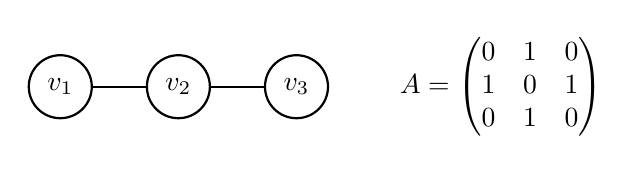
\begin{tikzpicture}[thick,every node/.style={circle,draw,fill=white,minimum size=8mm}]
\node (v1) at (0,0) {$v_1$}; \node (v2) at (1.5,0) {$v_2$}; \node (v3) at (3,0) {$v_3$};
\draw (v1)--(v2)--(v3);
\node[draw=none,rectangle] at (5.6,0) {$A=\begin{pmatrix}0&1&0\\1&0&1\\0&1&0\end{pmatrix}$};
\end{tikzpicture}
\caption{The adjacency matrix records exactly which vertex pairs share an edge.}
\end{figure}

\begin{theorem}
For every integer $k\geq 1$, the entry $(A^k)_{ij}$ counts walks of length exactly $k$ from $v_i$ to $v_j$.
\end{theorem}
\begin{figure}[htbp]
\centering
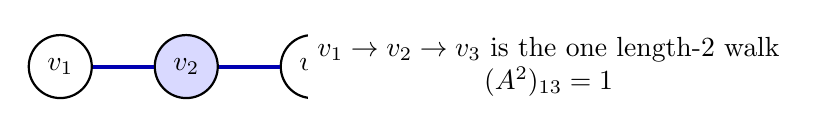
\begin{tikzpicture}[thick,every node/.style={circle,draw,fill=white,minimum size=8mm}]
\node (v1) at (0,0) {$v_1$}; \node[fill=blue!15] (v2) at (1.6,0) {$v_2$}; \node (v3) at (3.2,0) {$v_3$};
\draw[blue!70!black,line width=1.4pt] (v1)--(v2)--(v3);
\node[draw=none,rectangle,align=center] at (6.2,0) {$v_1\to v_2\to v_3$ is the one length-2 walk\\$(A^2)_{13}=1$};
\end{tikzpicture}
\caption{The intermediate vertex $v_2$ contributes one two-edge walk from $v_1$ to $v_3$.}
\end{figure}
\begin{proof}
For $k=1$, the entry $A_{ij}$ is 1 exactly when there is a one-edge walk. Suppose the statement holds for $k$. Then $(A^{k+1})_{ij}=\sum_m(A^k)_{im}A_{mj}$. For each intermediate vertex $v_m$, the product counts walks of length $k$ from $v_i$ to $v_m$ followed by the edge from $v_m$ to $v_j$. Summing over $m$ counts every walk of length $k+1$ exactly once.
\end{proof}

Important: powers count walks, not necessarily paths; walks may revisit vertices and edges. For instance, diagonal entries of $A^2$ count ways to leave a vertex and return in two steps.

\section*{\Enrichment{} Walk counts and linear recurrences}
A sequence $(a_n)$ satisfies a linear recurrence if each later term is a fixed linear combination of earlier terms. Walk counts in a fixed graph often follow such a rule. For the path $P_3$ with vertices $v_1-v_2-v_3$, let $a_n$ be the number of length-$n$ walks from $v_1$ to $v_2$. The first values are
\[
a_0=0,\quad a_1=1,\quad a_2=0,\quad a_3=2,\quad a_4=0,\quad a_5=4,\ldots
\]
Its adjacency matrix satisfies $A^3=2A$, so multiplying by further powers of $A$ shows $A^{n+2}=2A^n$ for $n\geq 1$. Therefore these walk counts obey $a_{n+2}=2a_n$ for $n\geq 1$. The recurrence describes the sequence without listing every walk.

\textbf{Explore.} Verify $A^3=2A$ for $P_3$, then use the recurrence to find the number of length-9 walks from $v_1$ to $v_2$. Does the alternating pattern of zero and nonzero terms make sense from the graph?

\section*{Exercises}
\begin{enumerate}
\item Write the adjacency matrix of the path $v_1-v_2-v_3$.
\item In that graph, explain why $(A^2)_{11}=1$ even though there is no path of length 2 from $v_1$ back to itself under our no-repeated-vertices definition of a path.
\item What does the sum of row $i$ of $A$ equal?
\end{enumerate}

\part{Structure theorems}
\chapter{Trees and spanning trees}
\section*{A network without redundancy}
A connected network with no cycles has exactly one simple route between any two vertices. Such a network is called a tree. Trees arise in family histories, file systems, communication backbones and efficient ways of linking locations.

\begin{definition}
A \emph{tree} is a connected graph with no cycles. A \emph{forest} is a graph with no cycles; each of its connected components is a tree. A \emph{spanning tree} of a graph is a subgraph that is a tree and contains every vertex of the original graph. A \emph{leaf} (or \emph{pendant vertex}) is a vertex of degree 1.
\end{definition}

\begin{figure}[htbp]
\centering
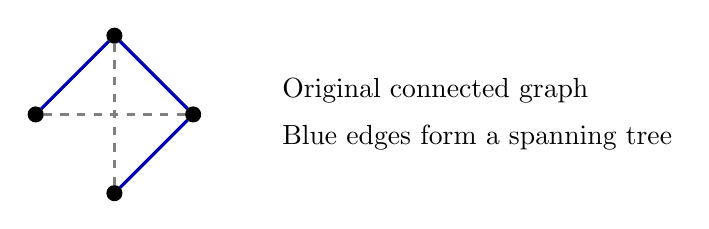
\begin{tikzpicture}[thick,vertex/.style={circle,draw=black,fill=black,inner sep=0pt,minimum size=5pt}]
\node[vertex] (a) at (0,0) {}; \node[vertex] (b) at (1,1) {}; \node[vertex] (c) at (2,0) {}; \node[vertex] (d) at (1,-1) {};
\draw[gray,dashed] (a)--(c) (b)--(d);
\draw[blue!70!black,line width=1.2pt] (a)--(b) (b)--(c) (c)--(d);
\node[draw=none,rectangle,fill=white,anchor=west] at (3,0.3) {Original connected graph};
\node[draw=none,rectangle,fill=white,anchor=west] at (3,-0.3) {Blue edges form a spanning tree};
\end{tikzpicture}
\caption{A spanning tree keeps every vertex while discarding cycle-forming edges.}
\end{figure}

\begin{theorem}[\Core{} Equivalent tree properties]
For a graph $T$ on $n\geq 1$ vertices, the following are equivalent: (i) $T$ is a tree; (ii) every pair of vertices is joined by a unique path; (iii) $T$ is connected and has $n-1$ edges; (iv) $T$ has no cycles and has $n-1$ edges.
\end{theorem}
\begin{figure}[htbp]
\centering
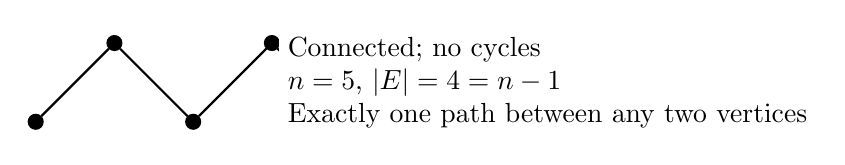
\begin{tikzpicture}[thick,vertex/.style={circle,draw=black,fill=black,inner sep=0pt,minimum size=5pt}]
\node[vertex] (a) at (0,0) {}; \node[vertex] (b) at (1,1) {}; \node[vertex] (c) at (2,0) {}; \node[vertex] (d) at (3,1) {}; \node[vertex] (e) at (4,0) {};
\draw (a)--(b)--(c)--(d)--(e);
\node[draw=none,rectangle,fill=white,align=left] at (6.5,0.5) {Connected; no cycles\\$n=5$, $|E|=4=n-1$\\Exactly one path between any two vertices};
\end{tikzpicture}
\caption{This five-vertex tree displays the equivalent edge-count and unique-path properties.}
\end{figure}
\begin{proof}
(i)$\Rightarrow$(ii): connectedness gives at least one path. If there were two different paths between the same vertices, follow them from their first divergence to their next meeting; together they contain a cycle. This contradicts that $T$ is acyclic.

(ii)$\Rightarrow$(i): a unique path for every pair gives connectedness. A cycle would give two different paths between two of its vertices, so there is no cycle.

For the edge count, use induction on $n$. A tree with at least two vertices has a leaf (an endpoint of a longest path; it cannot have another neighbour without extending the path or creating a cycle). Removing the leaf and its one edge leaves a tree. Induction gives $n-2$ remaining edges, so the original has $n-1$. Conversely, if a connected graph has more than $n-1$ edges, build a spanning tree by starting at one vertex and repeatedly adding an edge to a new vertex; this uses $n-1$ edges, so an extra edge closes a cycle. Hence a connected graph with $n-1$ edges is acyclic. Finally, an acyclic graph on $n$ vertices with $c$ components has $n-c$ edges, by applying the tree count to each component. If it has $n-1$ edges, then $c=1$, so it is connected. This proves all directions.
\end{proof}

\begin{example}[A five-site electricity backbone]
In a simplified model with five sites, any spanning tree uses exactly $5-1=4$ links. The tree connects all sites and contains no cycle, so it provides no alternative route if one of its links fails. This edge-count result says nothing about which four links are cheapest; assigning costs turns the problem into finding a minimum spanning tree, as in the optimisation chapter.
\end{example}

\begin{corollary}
Every tree with at least two vertices has at least two leaves. A forest with $n$ vertices and $k$ components has exactly $n-k$ edges.
\end{corollary}
\begin{proof}
The endpoints of a longest path in a tree are both leaves: an additional neighbour would either extend the path or create a cycle. For a forest, apply the tree edge count to each component and add: if their sizes are $n_1,\ldots,n_k$, the total number of edges is $\sum_{i=1}^k(n_i-1)=n-k$.
\end{proof}

\begin{proposition}
Every connected graph contains a spanning tree.
\end{proposition}
\begin{figure}[htbp]
\centering
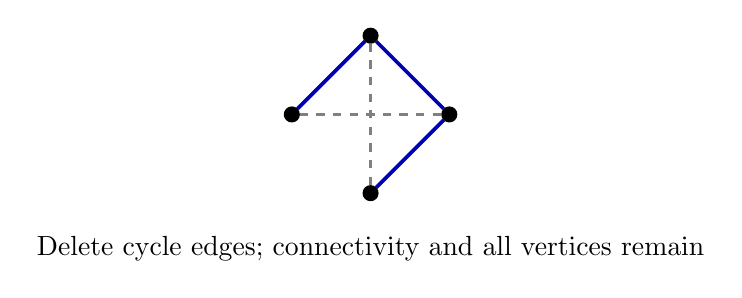
\begin{tikzpicture}[thick,vertex/.style={circle,draw=black,fill=black,inner sep=0pt,minimum size=5pt}]
\node[vertex] (a) at (0,0) {}; \node[vertex] (b) at (1,1) {}; \node[vertex] (c) at (2,0) {}; \node[vertex] (d) at (1,-1) {};
\draw[gray,dashed] (a)--(c) (b)--(d);
\draw[blue!70!black,line width=1.3pt] (a)--(b) (b)--(c) (c)--(d);
\node[draw=none,rectangle,fill=white] at (1,-1.7) {Delete cycle edges; connectivity and all vertices remain};
\end{tikzpicture}
\caption{Repeatedly deleting an edge from a cycle leaves a spanning tree.}
\end{figure}
\begin{proof}
If the graph has a cycle, delete one edge of that cycle; the graph remains connected, because the rest of the cycle still links the edge's endpoints. Repeat until no cycle remains. The resulting connected, acyclic spanning subgraph is a spanning tree.
\end{proof}

Adding one edge to a tree creates exactly one cycle: the new edge joins two vertices already joined by a unique tree path. Removing any edge from a tree disconnects it, since otherwise an alternate route would create a cycle.

\section*{An alkane's bond paths}
In 1875, Arthur Cayley used tree enumeration to count possible alkane structures (structural isomers), rather than to predict the existence of particular molecules.\footnote{A. Cayley, ``On the analytic forms called trees, with applications to the theory of chemical combinations,'' \emph{Report of the 45th Meeting of the British Association for the Advancement of Science} (1875), 257--305.} In a carbon skeleton, vertices represent carbon atoms and edges represent carbon--carbon bonds. Alkane carbon skeletons are trees; a cycle in the carbon skeleton instead indicates a cyclic hydrocarbon.

\begin{figure}[htbp]
\centering
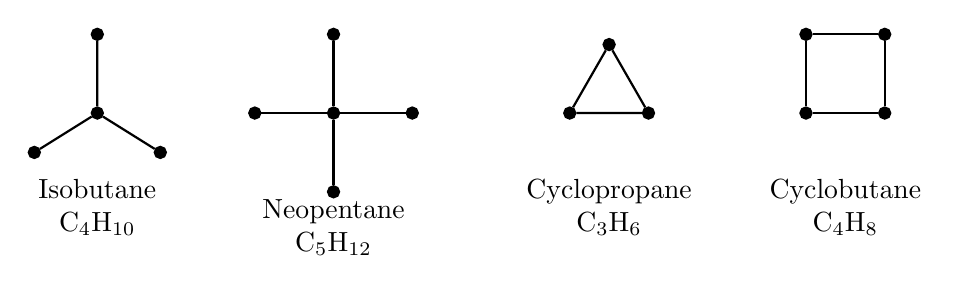
\begin{tikzpicture}[thick,carbon/.style={circle,draw=black,fill=black,inner sep=0pt,minimum size=4pt}]
\begin{scope}
\node[carbon] (i0) at (0,0) {};
\node[carbon] (i1) at (0,1) {};
\node[carbon] (i2) at (-0.8,-0.5) {};
\node[carbon] (i3) at (0.8,-0.5) {};
\draw (i0)--(i1) (i0)--(i2) (i0)--(i3);
\node[draw=none,align=center] at (0,-1.2) {Isobutane\\$\mathrm{C_4H_{10}}$};
\end{scope}
\begin{scope}[shift={(3,0)}]
\node[carbon] (n0) at (0,0) {};
\node[carbon] (n1) at (0,1) {};
\node[carbon] (n2) at (0,-1) {};
\node[carbon] (n3) at (-1,0) {};
\node[carbon] (n4) at (1,0) {};
\draw (n0)--(n1) (n0)--(n2) (n0)--(n3) (n0)--(n4);
\node[draw=none,align=center] at (0,-1.45) {Neopentane\\$\mathrm{C_5H_{12}}$};
\end{scope}
\begin{scope}[shift={(6,0)}]
\node[carbon] (p1) at (0,0) {};
\node[carbon] (p2) at (1,0) {};
\node[carbon] (p3) at (0.5,0.87) {};
\draw (p1)--(p2)--(p3)--(p1);
\node[draw=none,align=center] at (0.5,-1.2) {Cyclopropane\\$\mathrm{C_3H_6}$};
\end{scope}
\begin{scope}[shift={(9,0)}]
\node[carbon] (b1) at (0,0) {};
\node[carbon] (b2) at (1,0) {};
\node[carbon] (b3) at (1,1) {};
\node[carbon] (b4) at (0,1) {};
\draw (b1)--(b2)--(b3)--(b4)--(b1);
\node[draw=none,align=center] at (0.5,-1.2) {Cyclobutane\\$\mathrm{C_4H_8}$};
\end{scope}
\end{tikzpicture}
\caption{Carbon skeletons, with hydrogen atoms omitted. Isobutane and neopentane have tree-shaped carbon skeletons; cyclopropane and cyclobutane contain cycles and are cycloalkanes, not alkanes.}
\end{figure}

\Challenge{} \Uni{} \textbf{Problem.} The \emph{bond graph} of a chemical compound has one vertex per atom and one edge per bond. A hydrocarbon contains only carbon and hydrogen atoms. An alkane of order $n$ has formula $\text{C}_n\text{H}_{2n+2}$, and its bond graph $G$ is a tree in which each carbon vertex has degree 4 and each hydrogen vertex has degree 1. Suppose $E(G)$ is partitioned into $n+1$ edge-disjoint paths, each with two hydrogen endpoints.
\begin{enumerate}
\item Determine the maximum possible number of even-length paths in such a partition. Prove that this maximum can be achieved for every alkane of order $n$, regardless of its structural isomer.
\item Determine all positive integers $n$ for which $E(G)$ can be partitioned into $n+1$ paths that are all even in length.
\end{enumerate}

\begin{figure}[htbp]
\centering
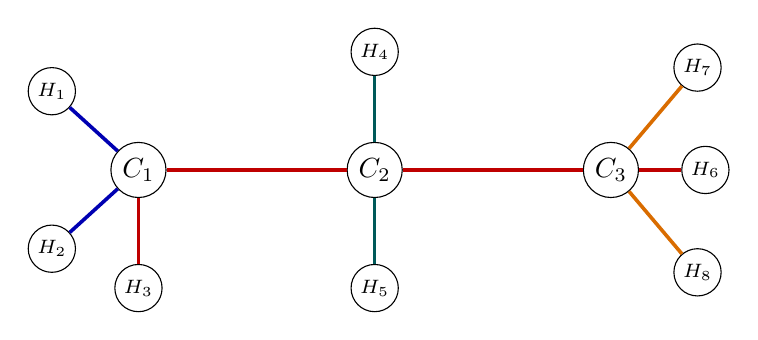
\begin{tikzpicture}[
carbon/.style={circle,draw=black,fill=white,minimum size=7mm,inner sep=1pt,font=\bfseries},
hydrogen/.style={circle,draw=black,fill=white,minimum size=6mm,inner sep=1pt,font=\scriptsize},
pathone/.style={blue!70!black,line width=1.3pt},
pathtwo/.style={red!75!black,line width=1.3pt},
paththree/.style={teal!70!black,line width=1.3pt},
pathfour/.style={orange!85!black,line width=1.3pt}]
\node[carbon] (c1) at (0,0) {$C_1$};
\node[carbon] (c2) at (3,0) {$C_2$};
\node[carbon] (c3) at (6,0) {$C_3$};
\node[hydrogen] (h1) at (-1.1,1) {$H_1$};
\node[hydrogen] (h2) at (-1.1,-1) {$H_2$};
\node[hydrogen] (h3) at (0,-1.5) {$H_3$};
\node[hydrogen] (h4) at (3,1.5) {$H_4$};
\node[hydrogen] (h5) at (3,-1.5) {$H_5$};
\node[hydrogen] (h6) at (7.2,0) {$H_6$};
\node[hydrogen] (h7) at (7.1,1.3) {$H_7$};
\node[hydrogen] (h8) at (7.1,-1.3) {$H_8$};
\draw[pathone] (c1)--(h1) (c1)--(h2);
\draw[pathtwo] (h3)--(c1)--(c2)--(c3)--(h6);
\draw[paththree] (c2)--(h4) (c2)--(h5);
\draw[pathfour] (c3)--(h7) (c3)--(h8);
\end{tikzpicture}
\caption{Propane's bond graph partitioned into four even paths: blue $H_1C_1H_2$ (length 2), red $H_3C_1C_2C_3H_6$ (length 4), teal $H_4C_2H_5$ (length 2), and orange $H_7C_3H_8$ (length 2).}
\end{figure}

\textbf{Solution.} There are $3n+2$ vertices in $G$, so the tree has $3n+1$ edges. The $n+1$ path lengths sum to $3n+1$. If $n$ is even, this sum is odd, so at least one path is odd and at most $n$ paths are even. If $n$ is odd, the edge count is even, giving the upper bound $n+1$. We construct partitions attaining these bounds for every alkane tree.

\textbf{Odd $n$.} Delete the hydrogen leaves to obtain the carbon skeleton $T_C$, a tree on $n$ vertices. Properly two-colour it with classes $X$ and $Y$. Let $H_X$ and $H_Y$ be the hydrogen leaves attached to carbon vertices in $X$ and $Y$, respectively. Since the bond graph is bipartite, the unique path between two hydrogen leaves has even length exactly when both lie in $H_X$ or both lie in $H_Y$.

Label every carbon--hydrogen edge by the colour of its carbon endpoint. For a carbon--carbon edge $uv$, deleting it from $T_C$ gives two subtrees; as $n$ is odd, exactly one has an odd number of vertices. Label $uv$ by the colour of the endpoint in that odd-sized subtree.

At any carbon vertex $w\in X$, deleting $w$ from $T_C$ gives branches $T_1,\ldots,T_k$, where $k=\deg_{T_C}(w)$. The carbon--carbon edge leading to $T_i$ has label $Y$ exactly when $|V(T_i)|$ is odd. Since these branch sizes sum to $n-1$, an even number of them are odd. Thus an even number of the carbon--carbon edges at $w$ have label $Y$. All $4-k$ carbon--hydrogen edges at $w$ have label $X$, so the number of incident edges of each label is even. The same argument with $X$ and $Y$ interchanged applies when $w\in Y$.

At each carbon, pair incident edges with the same label. Following these local pairings partitions all edges into paths: acyclicity rules out closed circuits, and the unpaired endpoints are precisely the hydrogen leaves. Hence there are $(2n+2)/2=n+1$ paths. Along any one path, all edges have the same label; its endpoint leaves therefore both belong to $H_X$ or both to $H_Y$. Each path has even length. This proves the bound $n+1$ for every odd-order alkane tree.

\textbf{Even $n$.} Choose a hydrogen leaf $h_0$ adjacent to a carbon $c_0$. Replace $h_0$ by a new carbon $c_{n+1}$ adjacent to $c_0$ and to three new hydrogen leaves $h_1,h_2,h_3$. The result is an alkane tree $G'$ of odd order $n+1$. Apply the odd-order construction. In its edge labelling, all four edges incident with $c_{n+1}$ have the same label: its carbon--carbon edge is labelled by the colour of $c_{n+1}$, since its side of the carbon skeleton has one vertex, and its three carbon--hydrogen edges receive that colour by definition. We may therefore choose the local pairing there so that $c_{n+1}h_1$ is paired with $c_{n+1}h_2$, and $c_0c_{n+1}$ is paired with $c_{n+1}h_3$.

The resulting even-path partition of $G'$ contains the path $h_1c_{n+1}h_2$ of length 2 and another even path $P$ containing the segment $c_0c_{n+1}h_3$. Delete the first path, and in $P$ replace that two-edge segment by the original edge $c_0h_0$. This shortens $P$ by one, making it odd; the other $n$ paths remain even. These paths partition $E(G)$, so the upper bound of $n$ even paths is attained for every even-order alkane tree.

Consequently,
\[
\max\{\text{number of even paths}\}=
\begin{cases}
n+1,&n\text{ odd},\\
n,&n\text{ even}.
\end{cases}
\]
All $n+1$ paths can be even exactly when $n$ is odd.

\textbf{Structural check.} If $|X|=x$ and $|Y|=y$, then $\sum_{v\in X}\deg_{T_C}(v)=n-1$, so $|H_X|=4x-(n-1)=4x-n+1$; similarly, $|H_Y|=4y-n+1$. Both counts are even exactly when $n$ is odd. The local edge pairings above use the tree structure to turn this parity into an actual path partition.

\section*{A challenge beyond alkane trees}
The previous challenge used the tree structure of alkanes. The next problem allows cycles in the carbon skeleton and combines the handshaking lemma with a double count of triangle--edge incidences.

\Challenge{} \Uni{} \textbf{Problem.} A \emph{saturated hydrocarbon graph} of formula $\mathrm{C}_n\mathrm{H}_m$ ($n,m\geq1$) is a finite simple connected graph $G=(V,E)$ whose vertex set is partitioned into a set $C$ of $n$ carbon vertices and a set $H$ of $m$ hydrogen vertices, such that every $c\in C$ has degree 4 and every $h\in H$ has degree 1. Assume that $H$ is independent (no two vertices of $H$ are adjacent) and that $G$ contains no clique $K_4$. A clique is a set of pairwise adjacent vertices; a clique of size 3 is called a triangle. Let $t$ be the number of triangles in $G$. For an independent set $I\subseteq V$, prove the following and answer the existence question:
\begin{enumerate}
\item Prove that $m$ is even and that
\[
24|I|+2t\leq 12n+21m.
\]
\item Determine all non-negative integers $t$ for which equality can hold for some saturated hydrocarbon graph and some independent set $I$.
\end{enumerate}

\textbf{Solution.} By the handshaking lemma,
\[
4n+m=\sum_{v\in V}\degG(v)=2|E|,
\]
so $m$ is even.

For the inequality, write $I_C=I\cap C$ and $I_H=I\cap H$, and let $E'$ be the set of edges with both endpoints in $V\setminus I$. Since $I$ is independent, every edge outside $E'$ is incident with exactly one vertex of $I$. Therefore
\[
|E|=4|I_C|+|I_H|+|E'|=4|I|-3|I_H|+|E'|,
\]
and hence
\[
4|I|+|E'|=|E|+3|I_H|
\leq \frac{4n+m}{2}+3m
=2n+\frac{7m}{2}.
\]
Multiplying by 6 gives
\[
24|I|+6|E'|\leq 12n+21m. \tag{1}
\]

Let $\mathcal{T}$ be the set of triangles, and count pairs $(e,T)$ with $e\in E'$ an edge of $T$. Each triangle contains at most one vertex of $I$, so it contains at least one edge of $E'$; thus there are at least $t$ such pairs. If an edge $e=xy$ lies in a triangle, then $x,y$ are carbon vertices, since hydrogen vertices have degree 1. The edge $xy$ can belong to at most three triangles, one for each possible common neighbour among the other neighbours of $x$ and $y$. Thus the number of pairs is at most $3|E'|$, and
\[
t\leq 3|E'|,\qquad 2t\leq 6|E'|. \tag{2}
\]
Combining (1) and (2) proves the result. The $K_4$-free condition is not needed for this bound, but it must hold in the examples attaining equality.

For equality, both bounds in the chain must be equalities. In particular, $t=3|E'|$, so $t$ is divisible by 3. Equality in (1) also requires $I_H=H$; equality in the incidence count means each triangle contains exactly one edge of $E'$ and each edge of $E'$ lies in exactly three triangles.

Conversely, let $t=3k$ for a non-negative integer $k$. If $k=0$, take methane: the star $K_{1,4}$ with its centre carbon and four hydrogen leaves, and let $I=H$. Then $n=1$, $m=4$, and equality holds.

For $k\geq1$, take carbon vertices $x_i,y_i$ for $1\leq i\leq k$ and $z_j$ for $1\leq j\leq 2k+1$. Add the edge $x_iy_i$ and join both $x_i$ and $y_i$ to each of $z_{2i-1},z_{2i},z_{2i+1}$. Each $x_i,y_i$ has degree 4. Every interior odd-indexed vertex $z_{2i+1}$ is shared by consecutive pairs and has degree 4; the remaining $k+2$ vertices $z_1,z_{2k+1},z_2,z_4,\ldots,z_{2k}$ have degree 2. To each of these remaining vertices attach two new carbon vertices, each joined to that $z$ and to three new hydrogen leaves. All vertices now have the required degrees. The construction is connected; its only triangles are $\{x_i,y_i,z_{2i-1}\}$, $\{x_i,y_i,z_{2i}\}$, and $\{x_i,y_i,z_{2i+1}\}$ for each $i$, so it is $K_4$-free.

Let $I$ consist of all the $z_j$ and all the hydrogen vertices. These vertices form an independent set, and the only edges with both endpoints outside $I$ are the $k$ edges $x_iy_i$. The graph has
\[
n=2k+(2k+1)+2(k+2)=6k+5,\qquad m=6(k+2)=6k+12,
\]
and $|I|=(2k+1)+m=8k+13$, while it has $t=3k$ triangles. Therefore
\[
24|I|+2t=24(8k+13)+6k=198k+312
=12(6k+5)+21(6k+12)=12n+21m.
\]
Thus equality is possible exactly for the non-negative multiples of 3.

\section*{Exercises}
\begin{enumerate}
\item A tree has 17 vertices. How many edges? If it has 12 edges, how many vertices?
\item Prove that every tree with at least two vertices has at least two leaves.
\item A connected graph has 8 vertices and 10 edges. How many edges must be removed to leave a spanning tree?
\item Explain why a tree with at least two vertices cannot have a universal vertex unless it is a star.
\end{enumerate}

\chapter{Eulerian and Hamiltonian problems}
\section*{One trip, every road}
An Euler trail uses every edge exactly once. It may begin and end at different vertices. An Euler circuit is a closed Euler trail. A graph with at least one edge is \emph{Eulerian} if it has an Euler circuit; isolated vertices are allowed. The distinction between covering edges and covering vertices is fundamental.

\begin{theorem}[\Core{} Euler criterion]
A connected graph with at least one edge has an Euler circuit if and only if every vertex has even degree. It has an open Euler trail if and only if exactly two vertices have odd degree.
\end{theorem}
\begin{figure}[htbp]
\centering
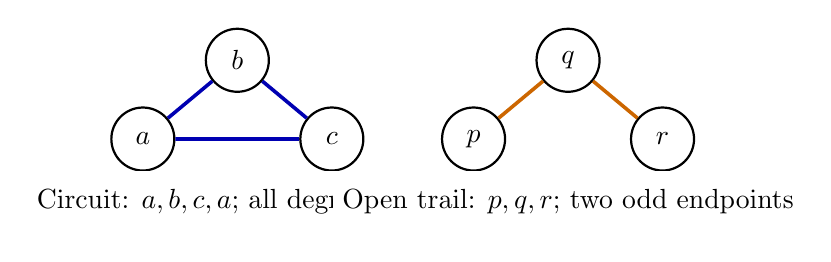
\begin{tikzpicture}[thick,every node/.style={circle,draw,fill=white,minimum size=8mm}]
\node (a) at (0,0) {$a$}; \node (b) at (1.2,1) {$b$}; \node (c) at (2.4,0) {$c$};
\draw[blue!70!black,line width=1.3pt] (a)--(b)--(c)--(a);
\node[draw=none,rectangle] at (1.2,-0.8) {Circuit: $a,b,c,a$; all degrees even};
\node (p) at (4.2,0) {$p$}; \node (q) at (5.4,1) {$q$}; \node (r) at (6.6,0) {$r$};
\draw[orange!80!black,line width=1.3pt] (p)--(q)--(r);
\node[draw=none,rectangle] at (5.4,-0.8) {Open trail: $p,q,r$; two odd endpoints};
\end{tikzpicture}
\caption{Euler circuits have no odd-degree vertices; open Euler trails have exactly two.}
\end{figure}
\begin{proof}
In any trail, each time the trail enters a vertex it must leave along a different unused edge. In a closed trail, these arrivals and departures pair up at every vertex, so all degrees are even. In an open trail, the start has one extra departure and the end one extra arrival, so precisely those two vertices have odd degree.

For sufficiency in the all-even case, start at any vertex and follow unused edges until no continuation is possible. At any vertex other than the start, arriving uses one edge, so an unused exit remains whenever the walk has not exhausted that vertex's incident edges. Thus the walk closes at its start. If unused edges remain, connectedness ensures some vertex on the closed walk is incident with an unused edge. Starting there, construct another closed trail of unused edges and splice it into the first. Repeat; finiteness ensures termination with an Euler circuit.

If exactly two vertices are odd, add one extra edge between them. The augmented graph is connected and all-even, so it has an Euler circuit. Removing the added edge leaves an Euler trail with the two odd vertices as endpoints. The necessary parity argument shows no other cases are possible.
\end{proof}

The connectedness condition matters: two disjoint cycles have only even degrees but no single walk can cover both. Isolated vertices can be disregarded if the graph has edges, but all non-isolated vertices must lie in one component.

A practical construction is Hierholzer's method: follow unused edges until returning to the start, then splice in further closed trails wherever unused edges remain. Fleury's rule (avoid a bridge unless forced) is another hand method, though it is less efficient.

A \emph{Hamiltonian path} is a path that visits every vertex exactly once. A \emph{Hamiltonian cycle} visits every vertex exactly once before returning to its start, and a graph containing one is called a \emph{Hamiltonian graph}. Unlike Euler circuits, there is no simple degree-parity test that characterises Hamiltonian graphs. A necessary condition is that every vertex have degree at least 2, but this is not sufficient: two triangles joined by a single bridge have minimum degree (the smallest vertex degree) 2 and no Hamiltonian cycle.

\begin{figure}[htbp]
\centering
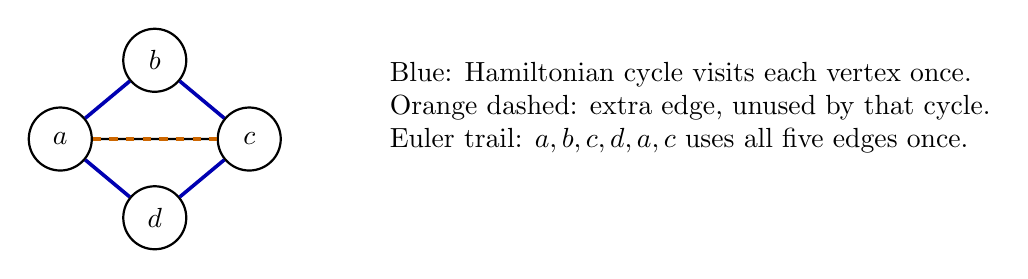
\begin{tikzpicture}[thick,every node/.style={circle,draw,fill=white,minimum size=8mm}]
\node (a) at (0,0) {$a$}; \node (b) at (1.2,1) {$b$}; \node (c) at (2.4,0) {$c$}; \node (d) at (1.2,-1) {$d$};
\draw (a)--(b)--(c)--(d)--(a) (a)--(c);
\draw[blue!70!black,line width=1.3pt] (a)--(b)--(c)--(d)--(a);
\draw[orange!80!black,line width=1.1pt,dashed] (a)--(c);
\node[draw=none,rectangle,align=left] at (8,0.4) {Blue: Hamiltonian cycle visits each vertex once.\\Orange dashed: extra edge, unused by that cycle.\\Euler trail: $a,b,c,d,a,c$ uses all five edges once.};
\end{tikzpicture}
\caption{Hamiltonian cycles cover vertices once; Euler trails cover edges once.}
\end{figure}

\Challenge{} The travelling salesperson problem asks for a minimum-weight Hamiltonian tour. Its optimisation version seeks the best tour; its decision version asks whether a tour of weight at most $B$ exists. No known algorithm solves all instances in time polynomial in the input size, but that is not a proof that no such algorithm exists.

\Challenge{} \textbf{Ore's theorem.} If $G$ has $n\geq 3$ vertices and every pair of nonadjacent vertices $u,v$ satisfies $\degG(u)+\degG(v)\geq n$, then $G$ has a Hamiltonian cycle.

\section*{Exercises}
\begin{enumerate}
\item Can a graph have exactly one odd-degree vertex? Why?
\item A connected graph has vertex degrees $2,2,4,4,2$. Does it have an Euler circuit? Explain.
\item Draw a connected graph with exactly two odd-degree vertices and give an Euler trail.
\item Give a connected graph where every vertex has degree at least 2 but no Hamiltonian cycle.
\item \Challenge{} Work through a proof of Ore's theorem. Suppose $u,v$ are nonadjacent and $\degG(u)+\degG(v)\geq n$. (a) If a Hamiltonian cycle in $G+uv$ avoids $uv$, explain why it is already in $G$; otherwise, delete $uv$ to obtain a Hamiltonian path $u=w_1,w_2,\ldots,w_n=v$ in $G$. (b) For $1\leq i\leq n-1$, let $I$ contain the indices for which $uw_{i+1}$ is an edge, and let $J$ contain those for which $w_iv$ is an edge. Explain why $|I|=\degG(u)$ and $|J|=\degG(v)$. (c) Since there are only $n-1$ indices, show that $I$ and $J$ overlap. Use an index in their intersection to rearrange the path edges into a Hamiltonian cycle in $G$. (d) Explain why adding such edges preserves the degree-sum condition for remaining nonadjacent pairs, and repeatedly add edges to deduce Ore's theorem.
\end{enumerate}

\chapter{Planarity and Euler's formula}
\section*{Can the connections avoid crossings?}
A graph is planar if it can be drawn in the plane with edges meeting only at common endpoints. A crossing in one drawing does not prove non-planarity: the graph may have another crossing-free drawing. A planar drawing divides the plane into regions called faces, including the unbounded outside face.

\begin{figure}[htbp]
\centering
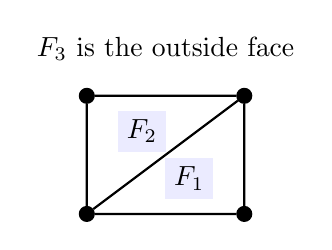
\begin{tikzpicture}[thick,vertex/.style={circle,draw=black,fill=black,inner sep=0pt,minimum size=5pt}]
\node[vertex] (a) at (0,0) {}; \node[vertex] (b) at (2,0) {}; \node[vertex] (c) at (2,1.5) {}; \node[vertex] (d) at (0,1.5) {};
\draw (a)--(b)--(c)--(d)--(a) (a)--(c);
\node[draw=none,rectangle,fill=blue!8] at (1.3,0.45) {$F_1$};
\node[draw=none,rectangle,fill=blue!8] at (0.7,1.05) {$F_2$};
\node[draw=none,rectangle,fill=white] at (1,2.1) {$F_3$ is the outside face};
\end{tikzpicture}
\caption{A crossing-free drawing has three faces: two inside and one outside.}
\end{figure}

\begin{theorem}[\Core{} Euler's formula]
For a connected planar graph with $v$ vertices, $e$ edges and $f$ faces, $v-e+f=2$.
\end{theorem}
\begin{figure}[htbp]
\centering
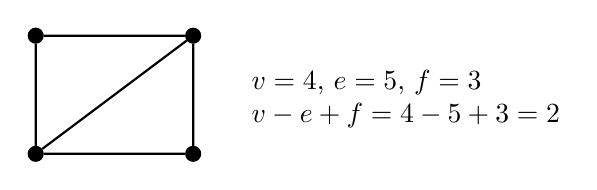
\begin{tikzpicture}[thick,vertex/.style={circle,draw=black,fill=black,inner sep=0pt,minimum size=5pt}]
\node[vertex] (a) at (0,0) {}; \node[vertex] (b) at (2,0) {}; \node[vertex] (c) at (2,1.5) {}; \node[vertex] (d) at (0,1.5) {};
\draw (a)--(b)--(c)--(d)--(a) (a)--(c);
\node[draw=none,rectangle,fill=white,align=left] at (4.7,0.7) {$v=4$, $e=5$, $f=3$\\$v-e+f=4-5+3=2$};
\end{tikzpicture}
\caption{Euler's formula counts vertices, edges, and faces in a planar embedding.}
\end{figure}
\begin{proof}
If the graph is a tree, it has $e=v-1$ and exactly one face, so $v-e+f=v-(v-1)+1=2$. Otherwise it contains a cycle. Delete an edge on a cycle. The graph stays connected, and the two faces on either side of that edge merge; thus $v$ decreases by 0, $e$ by 1 and $f$ by 1, leaving $v-e+f$ unchanged. Continue deleting cycle edges until a spanning tree remains. The tree case gives 2, so the original also gives 2.
\end{proof}

\Challenge{} If a plane graph has $c$ connected components, then
\[
v-e+f=1+c.
\]
To see this, first take a spanning forest: it has $v-c$ edges and one face. Adding each remaining edge within a component creates one cycle and splits one face into two, increasing both $e$ and $f$ by 1. Thus $v-e+f=v-(v-c)+1=1+c$.

For a simple connected planar graph with $v\geq 3$, each face boundary has at least three edge-sides, and each edge contributes two sides in total. Thus $3f\leq 2e$. Combining with Euler's formula gives $e\leq 3v-6$. If the graph is bipartite, every face boundary has at least four edge-sides, so $4f\leq 2e$ and $e\leq 2v-4$.

\Challenge{} The graph $K_5$ has $v=5,e=10$, exceeding $3v-6=9$, so it is not planar. The graph $K_{3,3}$ has $v=6,e=9$, exceeding the bipartite planar bound $2v-4=8$, so it too is non-planar.

\section*{\Challenge{} Stronger tests from faces}
The face-counting argument extends beyond triangular faces. The \emph{girth} of a graph is the length of its shortest cycle. If a connected simple planar graph has a cycle and girth $g\geq 3$, every face boundary has at least $g$ edge-sides. Since all $2e$ edge-sides are counted around faces, $gf\leq 2e$. Combining this with Euler's formula gives
\[
e\leq \frac{g}{g-2}(v-2).
\]
For $g=3$ this is the usual bound $e\leq 3v-6$; for a bipartite graph, $g\geq 4$ and it gives $e\leq 2v-4$. If the graph is a tree, the same bounds needed here follow directly from $e=v-1$.

This also gives an olympiad-style degree argument. A simple planar graph with $v\geq 3$ has a vertex of degree at most 5: otherwise every degree is at least 6, so the handshaking lemma gives $2e\geq 6v$, contradicting $e\leq 3v-6$. The argument applies to every subgraph as well, since subgraphs of planar graphs are planar.

\section*{\Uni{} Euler characteristic beyond the plane}
The planar formula is the genus-zero case of a broader topological statement. If a connected graph is embedded on an orientable surface of genus $h$ so that every face is a disk (a \emph{cellular embedding}), then
\[
v-e+f=2-2h.
\]
The sphere has genus $0$, giving Euler's formula; a torus has genus $1$, giving $v-e+f=0$. The term $2-2h$ is the Euler characteristic of the surface. This viewpoint is useful in university graph theory and topology; no surface theory is assumed elsewhere in this booklet.

For a connected simple graph with $v\geq 3$ cellularly embedded on this surface, counting at least three edge-sides around each face gives the corresponding bound $e\leq 3v-6+6h$ (with the tree case immediate). At genus zero this is the planar bound; increasing the genus allows more edges without crossings on the surface.

\textbf{Famous result (statement only).} Kuratowski's theorem says a finite graph is planar exactly when it contains no subdivision of $K_5$ or $K_{3,3}$. A subdivision replaces edges by internally vertex-disjoint paths; the theorem is not proved here.

\section*{Exercises}
\begin{enumerate}
\item A connected planar graph has 8 vertices and 12 edges. Find its number of faces.
\item Use the simple planar bound to show that $K_6$ is non-planar.
\item Why does a tree have one face when drawn in the plane without crossings?
\item \Challenge{} Show that every simple planar graph has a vertex of degree at most 5.
\end{enumerate}

\part{Colouring and optimisation}
\chapter{Graph colouring}
\section*{Avoiding clashes}
A proper vertex-colouring assigns colours to vertices so adjacent vertices receive different colours. The smallest number of colours needed is the chromatic number, written $\chiG(G)$. In a scheduling model, colours may represent time slots; in a map model, they may represent regions.

\begin{figure}[htbp]
\centering
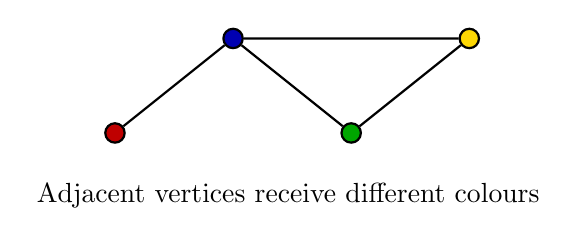
\begin{tikzpicture}[thick,vertex/.style={circle,draw=black,inner sep=0pt,minimum size=7pt}]
\node[vertex,fill=red!75!black] (a) at (0,0) {};
\node[vertex,fill=blue!70!black] (b) at (1.5,1.2) {};
\node[vertex,fill=green!65!black] (c) at (3,0) {};
\node[vertex,fill=yellow!75!orange] (d) at (4.5,1.2) {};
\draw (a)--(b)--(c)--(d) (b)--(d);
\node[draw=none,rectangle,fill=white] at (2.2,-0.8) {Adjacent vertices receive different colours};
\end{tikzpicture}
\caption{A proper colouring assigns different colours to the endpoints of every edge.}
\end{figure}

\begin{theorem}
A graph is bipartite if and only if it is 2-colourable (where a graph with no edges needs at most one colour).
\end{theorem}
\begin{proof}
If a graph is bipartite, give one colour to each vertex class. Conversely, the two colour classes of any proper 2-colouring contain no internal edges, so they form a bipartition.
\end{proof}

A greedy colouring processes vertices in some order, giving each the first colour not used by an already-coloured neighbour. If the maximum degree is $\Delta$, at most $\Delta$ colours are forbidden at any step, so $\Delta+1$ colours always suffice. The chosen order can make a big difference to how many colours greedy actually uses.

\begin{example}
For a triangle, greedy colouring requires three colours whatever the order, so $\chiG(K_3)=3$. For a path with at least one edge, alternating two colours works, and one cannot suffice, so its chromatic number is 2.
\end{example}

\begin{theorem}[\Challenge{} Five-colour theorem]
Every finite simple planar graph can be properly coloured with at most five colours.
\end{theorem}
\begin{proof}
We use induction on the number of vertices. The result is immediate for graphs with at most five vertices. For a planar graph with $n\geq 6$ vertices, Euler's planar edge bound implies that some vertex $v$ has degree at most 5: otherwise the degree sum would be at least $6n$, while $2m\leq 6n-12$. Remove $v$ and, by induction, colour the remaining graph with five colours. If $v$ has at most four neighbours, one of the five colours is available for it.

It remains to consider the case where $v$ has five neighbours. They cannot all be pairwise adjacent, since that would give a $K_5$ subgraph, contradicting the planar edge bound. Choose two nonadjacent neighbours $x$ and $y$. Contract the edges $vx$ and $vy$, merging $v,x,y$ into one vertex; remove any loops or duplicate edges that result. The resulting graph is still planar and has fewer vertices, so it has a proper colouring with five colours by induction. Give $x$ and $y$ the colour of the merged vertex. These two neighbours of $v$ now share a colour, so at most four colours appear on the five neighbours of $v$. Assign $v$ a fifth colour different from those. This extends the colouring to the original graph.
\end{proof}

The famous four-colour theorem improves the bound to four. Its first accepted proof was announced by Appel and Haken in 1976 and published in detail in 1977, with Part II coauthored by Koch; the proof used substantial computer assistance (Appel and Haken, 1976, 1977; Appel, Haken, and Koch, 1977).

\section*{\Enrichment{} Counting colourings}
The chromatic number records the fewest colours needed, but another question is how many proper colourings are possible. For a non-negative integer $q$, let $P_G(q)$ be the number of proper colourings of $G$ using a palette of $q$ labelled colours; colours in the palette need not all be used. As $q$ varies, this count is given by a polynomial, the \emph{chromatic polynomial}.

For a path $P_n$ on $n$ vertices, the first vertex has $q$ choices and each later vertex has $q-1$ choices, so
\[
P_{P_n}(q)=q(q-1)^{n-1}.
\]
For a cycle $C_n$ with $n\geq 3$, a standard count gives
\[
P_{C_n}(q)=(q-1)^n+(-1)^n(q-1).
\]
For example, a triangle has $P_{C_3}(q)=q(q-1)(q-2)$, as its three vertices must receive distinct colours. These formulas are optional extensions of chromatic number: they count all valid colourings, rather than only finding the minimum palette size.

\Uni{} For any edge $e$ of a simple graph $G$, deleting it gives $G-e$, while contracting its endpoints gives $G/e$. The deletion--contraction identity is
\[
P_G(q)=P_{G-e}(q)-P_{G/e}(q).
\]
Indeed, proper colourings of $G-e$ either give the endpoints of $e$ different colours (and hence colourings of $G$) or the same colour (counted by $G/e$). If contraction creates parallel edges, they impose the same colouring restriction and can be treated as one edge. This recursive method is a first taste of enumerative graph theory.

\section*{Exercises}
\begin{enumerate}
\item Find the chromatic numbers of $C_5$, $C_6$, and $K_4$.
\item Explain how to model exam scheduling as a colouring problem. What does a clique in the conflict graph tell you?
\item Prove that a graph containing a clique of size $r$ needs at least $r$ colours.
\item Find an ordering where greedy colouring uses more colours than necessary on a graph of your choice.
\end{enumerate}

\chapter{Optimisation and algorithms}
\section*{Routes and low-cost connectors}
A weighted graph assigns a number (such as distance, time or cost) to each edge. A shortest-path problem seeks a route of minimum total weight. In the Town Hall example, this means choosing a destination in the Blue Mountains and minimising the sum of the road-segment travel times. A minimum spanning tree (MST) seeks a least-total-weight set of edges connecting every vertex, without cycles. These are different questions: a shortest route between two points need not belong to every MST. The electricity-network example below is a deliberately simplified connectivity-and-cost model, not a design for the actual NSW grid.

\begin{figure}[htbp]
\centering
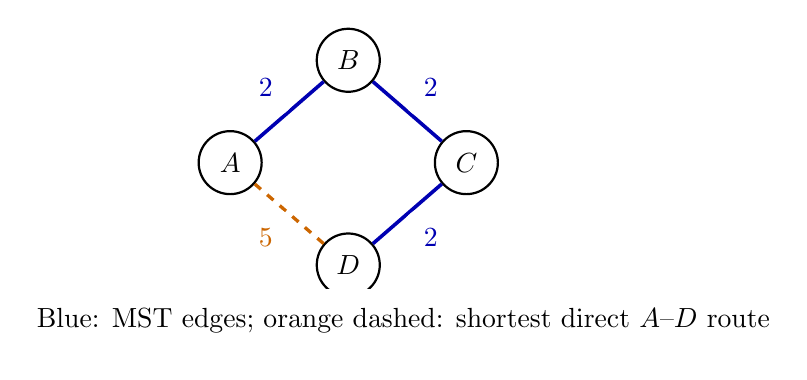
\begin{tikzpicture}[thick,every node/.style={circle,draw,fill=white,minimum size=8mm}]
\node (a) at (0,0) {$A$}; \node (b) at (1.5,1.3) {$B$}; \node (c) at (3,0) {$C$}; \node (d) at (1.5,-1.3) {$D$};
\draw[blue!70!black,line width=1.3pt] (a)--node[above left,draw=none,fill=white] {2} (b) (b)--node[above right,draw=none,fill=white] {2} (c) (c)--node[below right,draw=none,fill=white] {2} (d);
\draw[orange!80!black,dashed,line width=1.2pt] (d)--node[below left,draw=none,fill=white] {5} (a);
\node[draw=none,rectangle] at (2.2,-2) {Blue: MST edges; orange dashed: shortest direct $A$--$D$ route};
\end{tikzpicture}
\caption{The shortest route between two vertices and the minimum spanning tree solve different problems.}
\end{figure}

\section{A capacity-constrained delivery challenge}
\Challenge{} \Uni{} \textbf{Problem.} Suppose a town's two-way road network is a finite connected graph with positive road lengths. The inventory is at a vertex $O$, and there are $n$ delivery requests at vertices $P_1,\ldots,P_n$. Let $d$ denote shortest-path distance, let
\[
R=2\sum_{j=1}^n d(O,P_j)
\]
be the total distance for delivering every item separately, and let $W$ be the total length of all roads. A deliveryman can carry at most $k$ items per trip, where $k$ is a positive integer; every trip starts and ends at $O$. Prove that some delivery plan has total distance at most
\[
\frac{1}{k}R+\frac{2(k-1)}{k}W,
\]
and determine whether either coefficient can be decreased while the other is kept fixed.

\textbf{Solution.} First add requests at $O$ until the total number of requests is a multiple $km$ of $k$. These extra requests have zero travel cost and leave $R$ and $W$ unchanged, so removing them from any resulting plan gives a plan for the original requests with no greater distance. We may therefore work with $km$ requests.

Choose a shortest-path tree $T$ rooted at $O$. It is a subgraph of the road network, so its total length is at most $W$. Make a closed walk in $T$ that traverses each tree edge exactly twice, once in each direction. Its length is at most $2W$. List the requests $A_1,\ldots,A_{km}$ in the order their locations are first visited along this walk, listing requests at the same location consecutively, and put $A_{km+1}=A_1$. The shortest-path distance between consecutive locations is at most the length of the intervening part of the walk; for the final pair, use the end and beginning of the closed walk. Thus
\[
\sum_{i=1}^{km} d(A_i,A_{i+1})\leq 2W.
\]

For each of the $k$ cyclic shifts of this list, partition the requests into consecutive groups of $k$. Serve each group $A_i,\ldots,A_{i+k-1}$ on a trip that follows shortest paths from $O$ to $A_i$, between successive requests in the group, and from $A_{i+k-1}$ back to $O$. This is a feasible plan because the road network is undirected and each trip carries just its group's $k$ items.

Sum the lengths of all $k$ plans. Each request is the first in a group once and the last in a group once, so its radial path from and back to $O$ contributes $2d(O,A_i)$. The total radial contribution is therefore $R$. Each cyclic segment from $A_i$ to $A_{i+1}$ is internal to a group in $k-1$ shifts and is skipped at a group boundary in the other shift. The combined internal-segment contribution is at most
\[
(k-1)\sum_{i=1}^{km}d(A_i,A_{i+1})\leq 2(k-1)W.
\]
Hence the sum of the $k$ plan lengths is at most $R+2(k-1)W$. At least one plan has length no more than their average, giving the claimed bound.

Both coefficients are individually sharp. To see that $1/k$ cannot be lowered, fix $k$ and take a unit road $OX$, then attach $N=km$ distinct destinations to $X$ by separate spokes of length $\varepsilon=N^{-2}$. Then $W=1+N\varepsilon$, $R=2N(1+\varepsilon)$, and the optimal delivery distance $L_{\mathrm{opt}}$ is $2m+2N\varepsilon$: at least $m$ trips must each cross $OX$ out and back, and each short spoke must also be traversed twice. Grouping the destinations $k$ at a time attains this cost. As $m$ grows, $W$ stays near $1$, while $R/L_{\mathrm{opt}}\to k$. Thus any smaller coefficient of $R$, with the stated coefficient of $W$, eventually fails.

For the coefficient of $W$, take a star with centre $O$, $k$ unit-length spokes, and one request at the end of each spoke. Here $W=k$ and $R=2k$. Every spoke must be traversed twice, so the optimal total distance is $2k$. With the coefficient of $R$ fixed at $1/k$, any valid coefficient $\beta$ of $W$ must satisfy $2k\leq 2+\beta k$, or $\beta\geq 2(k-1)/k$. This includes $k=1$, when the sharp coefficient is $0$.

The averaging also explains the form of the bound: the total radial cost across the $k$ plans is always $R$, while the contribution from the closed tree walk is shared across those plans. For $k=1$ the bound is $R$; as capacity grows, it approaches the familiar tree-tour bound $2W$.

\section{Dijkstra's algorithm}
For a weighted graph with non-negative edge weights, Dijkstra's algorithm finds shortest-path distances from a chosen source $s$. It keeps a tentative distance $d(v)$ for each vertex and finalises these distances one at a time, from smallest to largest.

To find a shortest path from $s$ to a target $t$:
\begin{enumerate}
\item Set $d(s)=0$, set every other tentative distance to infinity, and leave all predecessor records empty.
\item Choose an unfinalised vertex $u$ with the smallest finite tentative distance and finalise it. If no such vertex remains, any unfinalised vertices are unreachable from $s$.
\item For each unfinalised neighbour $v$ of $u$, compare $d(u)+w(uv)$ with $d(v)$, where $w(uv)$ is the edge weight. If the new value is smaller, replace $d(v)$ with it and record $u$ as the predecessor of $v$.
\item Repeat until $t$ is finalised or no reachable unfinalised vertices remain. Follow predecessor records backwards from $t$ to recover the route.
\end{enumerate}

Here is a small illustrative model of the Town Hall question. The edge weights are illustrative travel times in minutes, not current route estimates. Let $H$ represent Town Hall, $M$ a chosen destination in the Blue Mountains, and $A,B$ intermediate road junctions. Starting at $H$, the algorithm first gives $A$ distance 2 and $B$ distance 5. After finalising $A$, it improves $B$ to 3 and gives $M$ distance 9. Finalising $B$ then improves $M$ to 5. Dijkstra's algorithm chooses $H$--$A$--$B$--$M$, with total time $2+1+2=5$ minutes; BFS chooses the two-edge route $H$--$B$--$M$, which takes $5+2=7$ minutes.

\begin{theorem}
Dijkstra's algorithm correctly computes shortest-path distances in a finite graph with non-negative edge weights.
\end{theorem}
\begin{figure}[htbp]
\centering
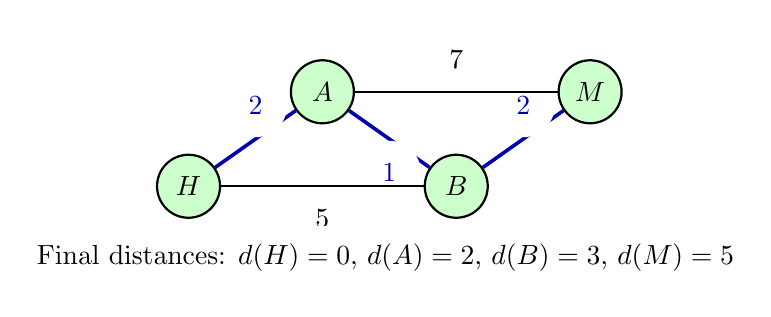
\begin{tikzpicture}[thick,every node/.style={circle,draw,fill=white,minimum size=8mm}]
\node[fill=green!20] (h) at (0,0) {$H$}; \node[fill=green!20] (a) at (1.7,1.2) {$A$};
\node[fill=green!20] (b) at (3.4,0) {$B$}; \node[fill=green!20] (m) at (5.1,1.2) {$M$};
\draw[blue!70!black,line width=1.3pt] (h)--node[above,draw=none,fill=white] {2} (a)--node[below,draw=none,fill=white] {1} (b)--node[above,draw=none,fill=white] {2} (m);
\draw (h)--node[below,draw=none,fill=white] {5} (b) (a)--node[above,draw=none,fill=white] {7} (m);
\node[draw=none,rectangle] at (2.5,-0.9) {Final distances: $d(H)=0$, $d(A)=2$, $d(B)=3$, $d(M)=5$};
\end{tikzpicture}
\caption{Illustrative travel times in minutes. $H$ is Town Hall, $M$ is a Blue Mountains destination, and $A,B$ are junctions.}
\end{figure}
\begin{proof}[Why the selection is safe]
Suppose $u$ is the unvisited vertex of smallest tentative distance. Any route to $u$ not already represented by a permanent vertex must reach some unvisited vertex first. The distance to that first unvisited vertex is at least the smallest tentative label, while the remaining edge weights are non-negative. Therefore no route through unvisited territory can reach $u$ with a smaller distance. So $u$'s label is final. Repeating this argument finalises every reachable vertex.
\end{proof}

Negative weights break the argument: a later route could reduce a distance after a vertex was marked permanent. For instance, an edge of weight $-5$ could make a route through an apparently longer intermediate vertex cheaper.

\section{Minimum spanning trees}
Kruskal's algorithm sorts edges from lightest to heaviest, adding an edge if it does not create a cycle. Prim's algorithm starts from one vertex and repeatedly adds a cheapest edge joining the current tree to a new vertex.

\begin{lemma}[Cut property]
For any cut (a partition of the vertices into two nonempty sets), a uniquely lightest edge crossing the cut belongs to every MST.
\end{lemma}
\begin{figure}[htbp]
\centering
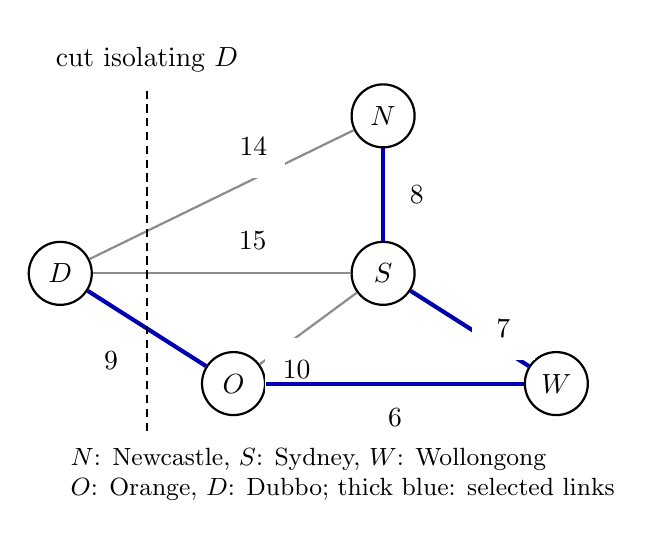
\begin{tikzpicture}[thick,every node/.style={circle,draw,fill=white,minimum size=8mm}]
\node (n) at (0.8,2) {$N$}; \node (s) at (0.8,0) {$S$};
\node (w) at (3,-1.4) {$W$}; \node (o) at (-1.1,-1.4) {$O$};
\node (d) at (-3.3,0) {$D$};
\draw[black!45] (d)--node[pos=.62,above,rectangle,text=black,draw=none,fill=white] {14} (n);
\draw[black!45] (s)--node[pos=.62,below,rectangle,text=black,draw=none,fill=white] {10} (o);
\draw[black!45] (d)--node[pos=.62,above,rectangle,text=black,draw=none,fill=white] {15} (s);
\draw[blue!70!black,line width=1.5pt] (o)--node[below,rectangle,text=black,draw=none,fill=white] {6} (w);
\draw[blue!70!black,line width=1.5pt] (s)--node[pos=.5,right,rectangle,text=black,draw=none,fill=white] {7} (w);
\draw[blue!70!black,line width=1.5pt] (s)--node[right,rectangle,text=black,draw=none,fill=white] {8} (n);
\draw[blue!70!black,line width=1.5pt] (d)--node[pos=.48,below left,rectangle,text=black,draw=none,fill=white] {9} (o);
\draw[black,densely dashed] (-2.2,-2.0)--(-2.2,2.55);
\node[draw=none,rectangle,fill=white] at (-2.2,2.72) {cut isolating $D$};
\node[draw=none,rectangle,align=left,anchor=west,font=\small] at (-3.3,-2.55) {$N$: Newcastle, $S$: Sydney, $W$: Wollongong\\$O$: Orange, $D$: Dubbo; thick blue: selected links};
\end{tikzpicture}
\caption{A fictional NSW-inspired network. Edge labels are invented cost units, and the schematic locations and links are not actual transmission routes.}
\label{fig:nsw-mst-model}
\end{figure}
\begin{proof}
If an MST omitted that edge, add it. This creates a cycle, which must contain another edge crossing the same cut. Removing that other, heavier edge leaves a spanning tree of smaller total weight, contradicting minimality.
\end{proof}

\begin{example}[A simplified electricity-link model]
Suppose the five labelled hubs and candidate links have the invented costs shown in Figure~\ref{fig:nsw-mst-model}. Kruskal accepts $OW=6$, $SW=7$, $SN=8$, and $OD=9$, connecting all five hubs with four links and total cost $30$. The cut isolating Dubbo is crossed by $OD=9$, $ND=14$, and $SD=15$. Since $OD$ is uniquely cheapest, the cut property guarantees that every MST contains it.
\end{example}

The tree selected above is the path $D$--$O$--$W$--$S$--$N$. If the design also requires protection from any one link failure, adding the candidate link $ND=14$ closes a cycle through all five hubs. The resulting five-link network costs $30+14=44$ and remains connected after deleting any one of those five links. This illustrates how a resilience requirement changes the optimisation question.

\Enrichment{} \textbf{Why Kruskal's algorithm works.} Adding an edge $e$ not in a spanning tree $T$ creates a cycle. Removing any other edge $f$ on that cycle gives another spanning tree, $T-f+e$; this is the edge-exchange lemma.

\begin{proof}[Correctness of Kruskal's algorithm]
The selected edges always form a forest. Since the original graph is connected, whenever this forest has more than one component there is an edge joining two of them; Kruskal eventually considers and accepts such an edge. Thus the algorithm ends with a spanning tree.

To see that it has minimum weight, start with any minimum spanning tree $T$ containing all edges Kruskal has selected so far; initially, any minimum spanning tree works. Let $e$ be the next edge selected. If $e$ is already in $T$, keep $T$. Otherwise, adding $e$ to $T$ creates a cycle. Since $e$ joins distinct components of the selected forest, that cycle contains another edge $f$ crossing the cut between the component containing one endpoint of $e$ and the rest. Every edge crossing this cut is eligible for addition to the selected forest, so Kruskal's choice gives $w(e)\leq w(f)$. Replacing $f$ by $e$ gives a spanning tree of no greater weight, hence another minimum spanning tree containing the longer selected prefix. Repeating proves that Kruskal's final tree is minimum.
\end{proof}

\Enrichment{} If all edge weights are distinct, the minimum spanning tree is unique. At each step, the next Kruskal edge is the uniquely lightest edge crossing the cut between one current forest component and the rest. By the cut property, every minimum spanning tree must contain it. This holds at every step, so every minimum spanning tree is Kruskal's tree.

\section{How algorithms scale}
An algorithm's input size grows with the number of vertices and edges. A method taking roughly $n^2$ elementary steps may be practical for hundreds or thousands of objects, while one taking roughly $2^n$ steps quickly becomes infeasible. This qualitative comparison is more useful than timing one small example on one computer.

\section*{Exercises}
\begin{enumerate}
\item Run Dijkstra's algorithm on a small weighted graph of your choice. Show each tentative-distance update.
\item Construct a graph with a negative edge for which Dijkstra's algorithm finalises an incorrect distance.
\item On the five-hub model in Figure~\ref{fig:nsw-mst-model}, run Prim's algorithm starting at Sydney and run Kruskal's algorithm. List the accepted links in order and find the total cost of the MST.
\item Explain why the cut property justifies a cheapest edge across a cut in an MST, but does not justify choosing each next edge greedily when constructing a travelling-salesperson tour.
\end{enumerate}

\chapter{Applications and investigations}
Graphs are useful not because every situation is literally a collection of dots and lines, but because they isolate relations that matter to a question. A strong investigation makes the modelling choices explicit, tests conjectures on small examples, and explains what a result means back in context.

\section{Applications: several kinds of networks}
The same graph ideas apply to very different networks. In each case, the model depends on the question: a link may be directed, weighted, or labelled, and the model should include only information needed to answer that question.

\subsection{Social networks}
Represent people by vertices and a relationship by an edge. Mutual friendships can be modelled by undirected edges, while following, messaging, or citing can be represented by directed edges. If interaction frequency matters, attach a weight to each edge. Degree can describe how many contacts a person has, while paths can describe chains of connection.

\textbf{Try it.} Model a small directed network of people who follow one another. Specify whether repeated interactions count, then design an algorithm that finds everyone reachable from a chosen person. Explain why the algorithm finds all and only those people by showing that each newly reached vertex is adjacent to one already reached.

\subsection{Transport networks}
Represent locations such as stations or intersections by vertices and direct routes by edges. A route may be directed, and its travel time, distance, or fare can be an edge weight. Shortest-path algorithms can then compare journeys, while a minimum spanning tree answers a different question: how to connect all locations at minimum total link cost.

\textbf{Try it.} Build a weighted transport network and construct a step-by-step method for finding a least-time route from a specified origin. State the condition on edge weights your method needs, and justify why its next choice cannot later be improved.

\subsection{A simplified electricity-link network}
Use the NSW-inspired five-hub model in Figure~\ref{fig:nsw-mst-model}. Its vertices are labelled Newcastle, Sydney, Wollongong, Orange and Dubbo; its edges are possible links, and the displayed values are invented cost units. For the deliberately limited objective of connecting all five hubs at minimum total cost, an MST is the right model: it uses four links and costs 30 units. The schematic is not a geographic map or a representation of existing transmission infrastructure. Real electricity-network design involves requirements beyond connectivity and minimum link cost, including reliability and capacity.

The MST is a path, so a single link failure can disconnect it. Adding the candidate link $ND$ of cost 14 closes a cycle through all five hubs. This five-link design costs 44 units and remains connected after any one of its links is removed.

\textbf{Try it.} Starting from the MST in Figure~\ref{fig:nsw-mst-model}, test each unused candidate link one at a time. Which addition makes the resulting network stay connected after any single link failure? Justify your answer by examining cycles, then explain what the toy model omits.

\subsection{Telecommunication networks}
Represent exchanges or relay stations by vertices and communication links by edges. Links may have costs or capacities. Connectivity asks whether messages can travel between sites; edge-disjoint paths ask whether communication can survive a link failure. A spanning tree gives a connected backbone without redundant links, while additional links may improve resilience.

\textbf{Try it.} For a proposed network, test whether it stays connected after any one link is removed. Turn your test into an algorithm and prove that it succeeds exactly when every pair of sites remains connected after each such removal.

\subsection{Computer networks}
Represent computers, routers, or servers by vertices and physical or logical connections by directed or undirected edges. Edge labels can record bandwidth, delay, or reliability. Reachability can model whether a device can send data to another; a flow model can represent how much data can be sent when links have capacity limits.

\textbf{Try it.} Give every link a capacity and design a procedure that repeatedly finds a source-to-destination augmenting path in the residual network (a path whose edges have positive residual capacity), then augments the flow by the path's bottleneck residual capacity. After each augmentation, decrease the residual capacity of every used residual edge by the augmentation amount and increase the capacity of its corresponding reverse residual edge; reverse edges record how much earlier flow can be cancelled. State and justify the stopping condition: no source-to-destination path remains in the residual network.

Across these settings, a sound algorithm description specifies its input, its steps, and when it stops. A correctness argument connects those steps to the model: an invariant explains what remains true during the procedure, and a final argument shows that the output answers the original question. State assumptions such as non-negative travel times or reliable links explicitly, since conclusions proved for the graph model hold in the real network only to the extent that the model is appropriate.

\subsection{Beyond communication networks}
Graph theory also appears in computer science, statistical physics, and computational biology. For example:
\begin{itemize}
\item \textbf{Computer science:} In a web of software dependencies, which package could break the most other programs if it fails?
\item \textbf{Statistical physics:} If particles affect only their neighbours, how can a tiny local change trigger a system-wide shift?
\item \textbf{Computational biology:} In a protein-interaction graph, which protein might be a crucial link in a biological process?
\end{itemize}

\section{An investigation cycle}
\begin{enumerate}
\item Ask a focused question. Example: how many links are needed to make a communication network robust to one failure?
\item Define the vertices, edges, and any weights or directions.
\item Explore small cases and record patterns.
\item State a conjecture precisely, including its assumptions.
\item Prove it or find a counterexample.
\item Interpret the result and discuss what the model leaves out.
\end{enumerate}

\section*{Two investigations in probability and counting}
\subsection*{Random graphs}
In the random graph model $G(n,p)$, begin with $n$ labelled vertices and independently include each possible edge with probability $p$. For example, when $n=5$ there are $\binom{5}{2}=10$ possible edges; if $p=\tfrac12$, each of the $2^{10}$ graphs is equally likely. The expected number of edges is $p\binom{n}{2}$, since each possible edge contributes probability $p$ of appearing.

\Investigation{} Generate several $G(n,p)$ graphs, by hand for small $n$ or with a spreadsheet or short program. For fixed $n$, compare what happens as $p$ increases: how do the number of edges, largest degree, and connectedness change? Record variation between trials as well as the typical pattern. \Coding{} Try many trials and compare the average number of edges with $p\binom{n}{2}$; no programming language is required.

\subsection*{The party problem and Ramsey theory}
Colour each edge of a complete graph red or blue. The following small Ramsey result says that any such colouring of $K_6$ contains a monochromatic triangle; in a party model, red can mean ``know one another'' and blue ``do not know one another''.

\Challenge{} Choose one vertex $x$. Among its five incident edges, at least three have the same colour. If those three neighbours contain an edge of that colour, it forms a monochromatic triangle with $x$. If none does, the three neighbours form a monochromatic triangle in the other colour. Thus every red-blue colouring of $K_6$ contains a monochromatic $K_3$.

Six is the smallest number with this guarantee: colour the edges of a $K_5$ red around a 5-cycle and blue on the remaining edges. Both colours form 5-cycles, so neither contains a triangle. The least $N$ such that every red-blue colouring of $K_N$ contains a monochromatic $K_3$ is called the Ramsey number $R(3,3)$; the argument proves $R(3,3)=6$. General Ramsey theory studies how these guarantees grow for larger cliques and more colours; that broader theory is beyond this short enrichment.

\subsection*{An olympiad challenge: intersecting triangles}
\Challenge{} \textbf{Problem (IMO 2001 Shortlist).} Model the people at a party by the vertices of a simple graph $G$, joining two people when they know each other. A $k$-clique is a set of $k$ pairwise acquainted people. Suppose every pair of $3$-cliques has at least one person in common, and there is no $5$-clique. Prove that at most two people can be chosen so that, after they leave, no $3$-clique remains.

\textbf{Solution.} In graph language, $G$ has no $K_5$, and every two triangles intersect. We seek a set of at most two vertices that meets every triangle. If there are no triangles, the empty set works.

\textbf{Case 1: $G$ contains a $K_4$.} Let its vertices be $Q=\{a,b,c,d\}$. Every triangle must contain at least two vertices of $Q$: if it contained at most one, the other three vertices of $Q$ would form a triangle disjoint from it. Now consider the two pairs $\{a,b\}$ and $\{c,d\}$. If neither pair met every triangle, there would be a triangle avoiding $\{a,b\}$, necessarily of the form $\{c,d,x\}$, and a triangle avoiding $\{c,d\}$, necessarily of the form $\{a,b,y\}$. These triangles must intersect, so $x=y$. This vertex is adjacent to all four vertices of $Q$, creating a forbidden $K_5$. Thus one of the two pairs meets every triangle.

\textbf{Case 2: $G$ contains no $K_4$.} If every pair of triangles shares at least two vertices, choose one triangle $\{a,b,c\}$. Every triangle then contains at least two of these vertices, and so contains $a$ or $b$. The pair $\{a,b\}$ meets every triangle.

Otherwise, two triangles meet in exactly one vertex. Write them as $T_0=\{a,b,c\}$ and $T_1=\{a,d,e\}$. The vertex $a$ is adjacent to $b,c,d,e$. No triangle can lie among those four neighbours, since together with $a$ it would form a $K_4$. As $bc$ and $de$ are edges, the edges between $\{b,c\}$ and $\{d,e\}$ must form a matching: two such edges sharing an endpoint would create a triangle among the four neighbours.

Any triangle avoiding $a$ must meet both $T_0$ and $T_1$, so it contains one vertex from each of $\{b,c\}$ and $\{d,e\}$, and hence uses a cross-edge between these sets. Its third vertex lies outside $\{a,b,c,d,e\}$, since there is no triangle among the four neighbours.

If no triangle avoids $a$, then $\{a\}$ meets them all. Otherwise, if all triangles avoiding $a$ use just one cross-edge, say $bd$, then each contains $b$, and $\{a,b\}$ meets every triangle. If triangles avoiding $a$ use two cross-edges, they are disjoint, so after relabelling they are $bd$ and $ce$. Let the corresponding triangles be $T_2=\{b,d,x\}$ and $T_3=\{c,e,y\}$. Since every two triangles intersect and the pairs $\{b,d\}$ and $\{c,e\}$ are disjoint, we must have $x=y$. Any triangle avoiding $a$ uses either $bd$ or $ce$. In the first case it must intersect $T_3$ at $x$; in the second it must intersect $T_2$ at $x$. Thus every triangle either contains $a$ or contains $x$, and $\{a,x\}$ meets them all.

In either case, at most two vertices meet every triangle. Removing the corresponding people therefore leaves no $3$-clique.

\textbf{Takeaway.} The $K_4$ case uses complementary pairs: if both fail, they force a $K_5$. In the $K_4$-free case, the four neighbours of the bowtie's shared vertex induce a triangle-free graph, so the cross-edges form a matching. More generally, in a $K_t$-free graph, the common neighbourhood of a $K_r$ contains no $K_{t-r}$ for $r<t$; here this constrains the possible triangle overlaps and yields a two-vertex hitting set.

\section*{Investigation menu}
\begin{enumerate}
\item \Investigation{} \textbf{Friendship paradox.} In many social networks, a randomly chosen person's friends tend to have more friends than the person does. Build small graphs and compare the average degree of a randomly chosen vertex with the average degree seen by following a randomly chosen edge. Which assumptions matter?
\item \Investigation{} \textbf{Resilient connections.} For $n$ sites, what is the smallest number of edges that keeps the network connected after any single edge failure? Explore lower bounds and constructions.
\item \Investigation{} \textbf{Route planning.} Compare shortest routes and MSTs on maps you create. When do the objectives agree? When do they differ?
\item \Investigation{} \textbf{NSW-inspired electricity links.} In Figure~\ref{fig:nsw-mst-model}, begin with the MST and test each unused candidate link. Which single added link protects the network against any one link failure, and what is the total cost? Explain why the result is only a toy model of electricity-network planning.
\item \Investigation{} \textbf{Timetable design.} Create a conflict graph from a realistic set of subjects or activities. Compare a greedy schedule with a schedule using the fewest possible time slots.
\item \Investigation{} \textbf{Small-world networks.} Start with a ring, add a few long-range edges, and measure how typical distances change. Decide how to define ``typical'' and report your method.
\end{enumerate}

\section*{Communicating a graph argument}
A clear solution states the model, names the graph-theoretic claim, gives enough reasoning to justify the conclusion, and translates the answer back into the original setting. A diagram is helpful, but it does not replace proof when the question asks for a general result.

\chapter*{Conclusion}
\addcontentsline{toc}{chapter}{Conclusion}
Graph theory offers a compact language for studying connections, but its power comes from choosing a useful model and then reasoning carefully about its structure. The chapters in this booklet have introduced core ideas and proof techniques, alongside selected examples of how graphs support algorithms and applications. This draft gives priority to the theory; its problem collection is still developing.

\section*{Where to Go Next}
As the booklet grows, this section will point readers toward further topics and investigations. A natural next step is to revisit the chapter exercises, vary their assumptions, and create examples or counterexamples of your own. Future development will expand the problem sets and add supporting hints, worked solutions and takeaways, while retaining the theory as the foundation.

\appendix
\part{Applied networks}
\chapter{The school-course networks at a glance}
The core chapters develop graph theory as a mathematical subject. This appendix maps selected applied network techniques to the Australian senior mathematics course editions identified below. The mapping is not an assessment guide and was checked against the cited versions on 16 October 2026; consult the relevant authority for current requirements.

\begin{center}
\small
\begin{tabularx}{\textwidth}{>{\raggedright\arraybackslash}p{0.25\textwidth}*{3}{>{\raggedright\arraybackslash}X}}
\toprule
Topic & \shortstack[l]{NSW Standard\\(2024)} & \shortstack[l]{QCE General\\(2025 v1.3)} & \shortstack[l]{VCE General\\(Study Design 2023)}\\
\midrule
Routes, trees and shortest paths & Year 11: shortest routes and spanning trees [NSW11] & Unit 4 [QCE] & Unit 2: graphs and networks; Unit 4: Dijkstra [VCE2/VCE4]\\
Critical path analysis & Year 12 Standard 2 only [NSW12] & Unit 4 [QCE] & Unit 4 [VCE4]\\
Flow networks & Year 12 Standard 2 only [NSW12] & Unit 4 [QCE] & Unit 4 [VCE4]\\
Assignments & Not listed [NSW11, NSW12] & Unit 4, including the Hungarian method [QCE] & Unit 4, including assignment methods [VCE4]\\
\bottomrule
\end{tabularx}
\end{center}

The tags identify the syllabus scope summarized in the table: [NSW11] and [NSW12] refer to the NSW Mathematics Standard 11--12 Syllabus (2024), with [NSW12] restricted to Standard 2; [QCE] refers to QCAA General Mathematics 2025 v1.3; [VCE2] and [VCE4] refer to VCE General Mathematics Study Design 2023. Full source details and official links appear in ``Curriculum connections and sources.'' These are course connections, not prerequisites for the main text.

\chapter{Routes and minimal connectors}
\section{Shortest routes by inspection}
For a small network, list plausible routes and add their edge weights. Compare complete route totals, not the number of edges: a route with more edges can be shorter if those edges have smaller weights. [NSW11] [QCE] [VCE2/VCE4]

\section{Subgraphs}
Let $G=(V,E)$ be a graph, with each edge assigned its pair of endpoints. A graph $H=(V_H,E_H)$ is a \emph{subgraph} of $G$ if $V_H\subseteq V$, $E_H\subseteq E$, and both endpoints of every edge in $E_H$ belong to $V_H$. The endpoint assignment in $H$ is inherited from $G$. Thus, choosing a subset of edges also requires including their endpoints among the vertices; vertices or edges of $G$ may otherwise be omitted. In particular, a subgraph need not contain every edge of $G$ joining two vertices it retains.

\section{Minimum spanning trees}
A minimum spanning tree connects all listed locations at minimum total edge weight. Apply Prim's or Kruskal's algorithm (Chapter 8), making sure not to add an edge that closes a cycle. If some edge weights tie, there may be more than one MST, with the same minimum total weight. [NSW11] [QCE] [VCE4]

\section*{Exercises}
\begin{enumerate}
\item Design a weighted network with two different MSTs. Verify that their total weights agree.
\item Explain why finding the shortest route from a depot to each location separately is not necessarily the same as finding a minimum network that connects all locations.
\end{enumerate}

\chapter{Critical path analysis}
A project can be represented by activities and precedence constraints. In an activity-on-arrow network, arrows are activities and vertices are events. Each activity has a duration; an arrow points from the event that must occur first to the event that follows. A dummy activity, where used, has duration zero and records a precedence relation without consuming time.

Assume the network is a finite directed acyclic graph with one designated start event and one designated finish event, and that every event lies on a start-to-finish path. Use zero-duration dummy activities where needed to make the start and finish common to the project network. The recurrences below assume fixed, non-negative activity durations and no resource constraints. Define $E_j$ as the earliest event time of event $j$ and $L_j$ as its latest allowable event time without delaying the project. Set $E_{\text{start}}=0$ and evaluate
\[
E_j=\max_{i\to j}(E_i+d_{ij})
\]
for each other event $j$ in topological order, where $d_{ij}$ is the duration of activity $i\to j$. The project duration is $E_{\text{finish}}$.

Set $L_{\text{finish}}=E_{\text{finish}}$ and evaluate the backward recurrence in reverse topological order:
\[
L_i=\min_{i\to j}(L_j-d_{ij}).
\]
The latest start time of an activity $i\to j$ is $L_j-d_{ij}$. Its total float is latest start minus earliest start: $(L_j-d_{ij})-E_i$. Activities with zero float lie on at least one critical path. If any critical activity is delayed, the whole project is delayed unless the plan changes.

\begin{example}
Activity $A$ takes 3 days. After $A$, activities $B$ (2 days) and $C$ (5 days) run in parallel, then activity $D$ (1 day) follows both. The two route lengths are $3+2+1=6$ and $3+5+1=9$ days. The project takes 9 days; $A,C,D$ are critical, while $B$ has 3 days of float.
\end{example}

A Gantt chart places activities against a time axis and is useful for communicating a schedule. Crashing means shortening selected activity durations, usually at extra cost; the best choice targets critical work and accounts for how the critical path may change after an activity is shortened. [NSW12] [QCE] [VCE4]

\section*{Exercises}
\begin{enumerate}
\item In the example, calculate earliest and latest start times for each activity.
\item Give a precedence table with two critical paths. Explain what happens if one critical activity is shortened.
\item Why is an activity with positive float not necessarily irrelevant to project management?
\end{enumerate}

\chapter{Flow networks}
A flow network is a finite directed graph with distinct source $s$ and sink $t$, and a finite non-negative capacity $c(u,v)$ on every edge. A flow assigns a value $f(u,v)$ to each edge, satisfying $0\leq f(u,v)\leq c(u,v)$, and conserves flow at every vertex other than $s$ and $t$. Its value is the net outflow from the source,
\[
  |f|=\sum_{(s,v)\in E} f(s,v)-\sum_{(v,s)\in E} f(v,s).
\]
By conservation, this equals the net inflow at the sink.

A cut separates the vertices into a source side containing $s$ and a sink side containing $t$. Its capacity is the sum of capacities on edges directed from the source side to the sink side. The value of any flow is at most the capacity of every cut: flow conservation makes the net flow crossing the cut equal to the flow value, and each forward edge is capacity-limited.

\textbf{Max-flow min-cut theorem (statement).} In every finite capacitated network, the maximum possible flow value equals the minimum cut capacity. A constructive method repeatedly finds an augmenting path in the residual network. Residual edges record both unused capacity and the possibility of undoing earlier flow, which allows rerouting. Simply filling a locally available edge can miss the optimum.

For small networks, enumerate cuts to establish an upper bound, then exhibit a flow achieving that bound. The two matching values certify optimality. [NSW12] [QCE] [VCE4]

\section*{Exercises}
\begin{enumerate}
\item Give an example of a cut that proves a flow of value 8 is impossible.
\item Construct a small network where an early choice must be rerouted to obtain a maximum flow.
\item Explain why the capacity of a cut is an upper bound on any flow.
\end{enumerate}

\chapter{Assignment problems}
An assignment problem matches agents to tasks. Build a bipartite graph with one vertex class for agents and the other for tasks; an edge means the assignment is allowed. A matching is a set of edges with no shared endpoints. A perfect matching assigns every agent a distinct task.

For a weighted assignment, each allowed agent-task pair has a cost. The goal is to choose a perfect matching with minimum total cost. This is not the same as merely finding any perfect matching. The Hungarian algorithm solves weighted assignment problems systematically; for a small matrix, row and column reductions can help identify an optimum, but a valid solution must still assign each row and column exactly once and justify that no cheaper assignment exists. [QCE] [VCE4]

\Enrichment{} \textbf{Hall's marriage theorem.} A bipartite graph with vertex classes $U$ (agents) and $W$ (tasks) has a matching that assigns every vertex of $U$ to a different vertex of $W$ if and only if every subset $X\subseteq U$ has at least $|X|$ neighbours in $W$. Write $N(X)$ for the set of tasks adjacent to at least one agent in $X$; the condition is $|N(X)|\geq |X|$ for every $X\subseteq U$. When $|U|=|W|$, such a matching is perfect.

\begin{example}
For cost matrix $\begin{pmatrix}4&1&3\\2&0&5\\3&2&2\end{pmatrix}$, assigning row 1 to column 2, row 2 to column 1, and row 3 to column 3 has total cost $1+2+2=5$. Check the other possible permutations to determine whether this is optimal.
\end{example}

\section*{Exercises}
\begin{enumerate}
\item Use the example matrix to find the minimum assignment cost and an optimal assignment.
\item Give a bipartite graph with no perfect matching and explain the obstruction.
\item Explain why selecting the cheapest available task independently for each agent can fail.
\item \Enrichment{} Use Hall's theorem for these allowed assignments: $A$ may choose 1 or 2, $B$ may choose 1 or 2, $C$ may choose 2 or 3, and $D$ may choose 3 or 4. (a) Find a matching that assigns every agent a different task. (b) Change $C$'s choices to 1 or 2. For $X=\{A,B,C\}$, find $N(X)$ and compare $|N(X)|$ with $|X|$. (c) Explain why the modified choices cannot assign every agent a different task, even though each agent individually has options. (d) In your own words, describe what Hall's condition checks for a group of agents.
\end{enumerate}

\backmatter
\chapter*{Hints for challenging exercises}
\addcontentsline{toc}{chapter}{Hints for challenging exercises}
The hints below target proofs, challenge questions, enrichments, and tasks where choosing a useful construction is the main difficulty. Appendix references use the letters printed in the book: B for routes, C for critical path analysis, D for flows, and E for assignments.
\begin{description}[style=nextline]
\item[1.3] Compare degree sequences: they are preserved by isomorphism. Try a triangle with an isolated vertex and a star.
\item[2.1] A vertex cannot be adjacent to itself or to a second copy of the same neighbour.
\item[2.5] Count the vertex-edge incidences in two ways, then divide the total degree by 2.
\item[2.6] The reductions should be $3,3,2,2,2\to2,2,1,1\to1,1,0\to0,0$. Reversing each reduction tells you which edges to add.
\item[3.1] Repeat an edge for the walk that is not a trail; repeat a vertex but not an edge for the trail that is not a path.
\item[3.2] Use the theorem connecting bipartite graphs with odd cycles.
\item[3.4] Mark vertices when they are first discovered. A queue gives BFS; a stack (or recursion) gives DFS.
\item[4.2] Interpret the matrix entry as a two-step walk that leaves $v_1$ and returns to it.
\item[5.2] Take a path with the greatest possible number of vertices. What would an extra neighbour of either endpoint imply?
\item[5.3] A spanning tree on 8 vertices has a fixed number of edges. A connected graph can be reduced to one by deleting cycle edges.
\item[5.4] If the universal vertex is joined to all others, any extra edge among those others would make a cycle.
\item[6.1] Apply the handshaking lemma's corollary about the number of odd-degree vertices.
\item[6.4] Use two triangles joined by a single bridge; a cycle cannot use that bridge exactly once.
\item[6.5] For the Hamiltonian path, compare the two sets of indices in the question. Their sizes sum to more than the number of available indices.
\item[7.3] A tree has $e=v-1$. Substitute this into Euler's formula.
\item[7.4] Combine $e\leq3v-6$ with $\sum_v\degG(v)=2e$ and average the degrees.
\item[8.3] Every pair of vertices in the clique must receive distinct colours.
\item[8.4] Try the path $a-b-c-d$ in the order $a,d,b,c$.
\item[9.1] Choose a small graph with non-negative weights and show the labels after each vertex is made permanent.
\item[9.2] Let a vertex be settled before another vertex with a larger temporary label; then use a negative edge from the latter back to the settled vertex.
\item[9.3] Use the five-hub graph in the minimum-spanning-trees section. For Prim, start at Sydney and at each step choose the cheapest edge from the current tree to a new hub; for Kruskal, scan edges in increasing cost and skip any that closes a cycle.
\item[9.4] A locally cheapest tour edge can force an expensive final return. Compare a nearest-neighbour tour with another tour on four vertices.
\item[B.2] A triangle with all edge weights equal has three different spanning trees of equal total weight.
\item[C.2] Make two different start-to-finish routes have the same total duration.
\item[D.2] In the residual network, a reverse edge can undo an earlier assignment and free a route for another unit of flow.
\item[D.3] Sum the conservation equations over all vertices on the source side; internal edge flows cancel.
\item[E.3] Use a two-agent, two-task cost table where the cheapest choice for the first agent is the other agent's only inexpensive task.
\item[E.4] For the modified choices, take $X=\{A,B,C\}$ and list all tasks adjacent to at least one member of $X$.
\end{description}
\textbf{Challenge note (Ramsey problem in Chapter 10).} From one vertex of $K_6$, five edges have only two colours. Use the pigeonhole principle, then consider whether the three same-coloured neighbours contain an edge of that colour.

\chapter*{Answers and brief solutions}
\addcontentsline{toc}{chapter}{Answers and brief solutions}
For construction and modelling questions, the answer shown is one valid example; other correct models may differ. Proof questions receive a short argument or proof sketch. Appendix labels below match the printed chapter letters: Appendix B is routes, C is critical path analysis, D is flow networks, and E is assignments.

\section*{Chapter 1: Problems that lead to graphs}
\begin{description}[style=nextline]
\item[1.1] Use five vertices, one per person, and join two vertices if those people have exchanged a book. This simple graph forgets how many exchanges occurred, when they occurred, and which person initiated them.
\item[1.2] Use a directed graph, with an arc from a follower to the account followed. Give each arc a weight equal to the number of messages exchanged if message volume matters.
\item[1.3] Yes. A triangle plus an isolated vertex and the star $K_{1,3}$ each have four vertices and three edges, but their degree sequences differ.
\item[1.4] Make one vertex per exam and join two exams if at least one student must sit both. A proper colouring assigns non-conflicting time slots; the chromatic number is the minimum number of slots.
\end{description}

\section*{Chapter 2: Degrees, counting and proof}
\begin{description}[style=nextline]
\item[2.1] A vertex in a simple graph can be adjacent to at most the other $n-1$ vertices, so its degree is at most $n-1$.
\item[2.2] $K_{12}$ has $\binom{12}{2}=66$ edges; $K_{4,7}$ has $4\cdot7=28$ edges.
\item[2.3] Yes. The handshaking lemma gives total degree $2\cdot9=18$, so if every degree is 3 there must be $18/3=6$ vertices. Such a graph exists, for example the triangular prism.
\item[2.4] A path of length 2 has two edges but its two endpoints have degree 1, disproving the claim.
\item[2.5] The degree sum is $10\cdot3=30=2|E|$, so the Petersen graph has 15 edges.
\item[2.6] The reductions are $3,3,2,2,2\to2,2,1,1\to1,1,0\to0,0$, so the first sequence is graphical. One construction on vertices $A,B,C,D,E$ has edges $AB,AC,AD,BE,BC,DE$, giving degrees $3,3,2,2,2$. For $3,3,1,1$, the reductions reach $2,0,0$ and then force a negative degree, so it is not graphical.
\end{description}

\section*{Chapter 3: Paths and connectedness}
\begin{description}[style=nextline]
\item[3.1] On square $A-B-C-D-A$ with diagonal $AC$, $A-B-C-A-B$ is a length-4 walk that repeats edge $AB$. The walk $A-B-C-D-A$ is a trail but not a path because it repeats $A$.
\item[3.2] $C_7$ is not bipartite because it is an odd cycle. $C_{10}$ is bipartite by alternating the two classes around the even cycle.
\item[3.3] One example has components of sizes 1, 2, and 3: take an isolated vertex, a single edge, and a three-vertex path.
\item[3.4] The visit order depends on the chosen graph and neighbour order. BFS uses a queue and explores by distance; DFS uses a stack or recursion and follows one branch before backtracking.
\end{description}

\section*{Chapter 4: Matrices and graphs}
\begin{description}[style=nextline]
\item[4.1] The adjacency matrix is $\begin{pmatrix}0&1&0\\1&0&1\\0&1&0\end{pmatrix}$.
\item[4.2] $(A^2)_{11}=1$ counts the walk $v_1,v_2,v_1$. It is not a path because the starting vertex is repeated.
\item[4.3] The sum of row $i$ is the number of vertices adjacent to $v_i$, hence it equals $\degG(v_i)$.
\end{description}

\section*{Chapter 5: Trees and spanning trees}
\begin{description}[style=nextline]
\item[5.1] A tree on 17 vertices has 16 edges; a tree with 12 edges has 13 vertices, since every tree has one fewer edge than vertices.
\item[5.2] Choose a longest path in the tree. If an endpoint had a neighbour not on the path, the path could be extended; if it had another neighbour on the path, there would be a cycle. Thus both endpoints are leaves.
\item[5.3] A spanning tree on 8 vertices has 7 edges, so remove $10-7=3$ edges. Delete edges from cycles to preserve connectedness.
\item[5.4] If the universal vertex is joined to all other vertices, an edge between any two of the other vertices would form a triangle. Thus a tree with a universal vertex has only the universal vertex's incident edges: it is a star.
\end{description}

\section*{Chapter 6: Eulerian and Hamiltonian problems}
\begin{description}[style=nextline]
\item[6.1] No. The handshaking lemma implies that every graph has an even number of odd-degree vertices.
\item[6.2] Yes. The graph is connected and all listed degrees are even, so the Euler criterion gives an Euler circuit.
\item[6.3] A three-vertex path has degrees $1,2,1$ and has an Euler trail from one endpoint to the other.
\item[6.4] Take two triangles joined by one bridge. A Hamiltonian cycle would have to cross the bridge to enter and leave the other triangle, but there is only one such edge.
\item[6.5] If a Hamiltonian cycle in $G+uv$ uses $uv$, deleting it leaves a Hamiltonian path $w_1=u,\ldots,w_n=v$ in $G$. The sets $I$ and $J$ each index the neighbours of $u$ and $v$ along this path, so $|I|+|J|=\degG(u)+\degG(v)\geq n>n-1$. Hence they overlap at some $i$. The edges $uw_{i+1}$ and $w_iv$, together with the path edges, form a Hamiltonian cycle in $G$. Thus adding an edge between a nonadjacent Ore pair cannot create Hamiltonicity from nothing. Adding missing edges one at a time preserves the degree-sum condition; the complete graph is Hamiltonian, so reversing the additions proves $G$ is Hamiltonian.
\end{description}

\section*{Chapter 7: Planarity and Euler's formula}
\begin{description}[style=nextline]
\item[7.1] Euler's formula gives $f=2-v+e=2-8+12=6$.
\item[7.2] $K_6$ has 15 edges, exceeding the planar bound $3v-6=12$ for a simple planar graph on six vertices.
\item[7.3] A tree has $e=v-1$. Euler's formula then gives $f=2-v+(v-1)=1$.
\item[7.4] If every vertex had degree at least 6, the degree sum would give $2e\geq6v$. But planarity gives $e\leq3v-6$, hence $2e\leq6v-12$, a contradiction. Therefore some vertex has degree at most 5.
\end{description}

\section*{Chapter 8: Graph colouring}
\begin{description}[style=nextline]
\item[8.1] $\chiG(C_5)=3$, $\chiG(C_6)=2$, and $\chiG(K_4)=4$.
\item[8.2] Use one vertex per exam and an edge for each pair of exams sharing a student. A clique of size $r$ is a set of $r$ pairwise conflicting exams, so at least $r$ time slots are needed.
\item[8.3] Every two vertices in a clique are adjacent, so all $r$ vertices must receive distinct colours; at least $r$ colours are necessary.
\item[8.4] For path $a-b-c-d$, greedily colour in the order $a,d,b,c$. The first two get colour 1, then $b$ gets 2 and $c$ gets 3. Yet the path is bipartite and needs only 2 colours.
\end{description}

\section*{Chapter 9: Optimisation and algorithms}
\begin{description}[style=nextline]
\item[9.1] Example: use edges $SA=2$, $SB=5$, $AB=1$, $AT=6$, $BT=2$, with source $S$. After processing $S$, labels are $A=2,B=5$; processing $A$ updates $B=3,T=8$; processing $B$ updates $T=5$. The shortest distance to $T$ is 5 along $S-A-B-T$.
\item[9.2] Use directed edges $S\to A=2$, $S\to B=5$, $B\to A=-10$, $A\to T=2$, and $B\to T=1$. Dijkstra settles $A$ at 2 and can settle $T$ at 4 before $B$ at 5, but the actual route $S\to B\to A\to T$ has weight $-3$.
\item[9.3] Prim starting at $S$ accepts $SW=7$, $WO=6$, $SN=8$, and $OD=9$; the total is 30. Kruskal considers $WO=6$, $SW=7$, $SN=8$, and $OD=9$ in that order and accepts all four. Both produce the MST with four links, as expected for a tree on five vertices.
\item[9.4] The cut property supports an exchange proof for a spanning tree; it does not justify arbitrary next-edge choices in a tour. For example, on $K_4$ with $AB=BC=CD=1$, $AC=BD=2$, $DA=10$, nearest-neighbour starting at $A$ gives $A-B-C-D-A$ of weight 13, while $A-B-D-C-A$ has weight 6.
\end{description}

\section*{Appendix B: Routes and minimal connectors}
\begin{description}[style=nextline]
\item[B.1] A triangle with all three edge weights 2 has three distinct MSTs (each omits a different edge); each has total weight 4.
\item[B.2] On vertices $r,a,b$, set $ra=2$, $rb=2$, and $ab=1$. Shortest routes from $r$ to $a$ and $b$ use the two direct edges, total 4, while the MST uses $ra$ and $ab$, total 3. The objectives differ because shortest routes optimize origin-to-each distances, whereas an MST optimizes total connecting cost.
\end{description}

\section*{Appendix C: Critical path analysis}
\begin{description}[style=nextline]
\item[C.1] Earliest starts are $A=0$, $B=C=3$, $D=8$. Latest starts are $A=0$, $B=6$, $C=3$, $D=8$. Thus $A,C,D$ have zero float and $B$ has 3 days.
\item[C.2] For example, use two routes: $S\to A\to T$ with durations 2 and 3, and $S\to B\to T$ with durations 4 and 1. Both take 5 days. Shortening one activity on the first route leaves the second route at 5 days, so the project duration does not change; the second route becomes critical.
\item[C.3] An activity with float may use scarce people or equipment, face uncertainty, or become critical if another duration changes. Float is scheduling flexibility, not proof of irrelevance.
\end{description}

\section*{Appendix D: Flow networks}
\begin{description}[style=nextline]
\item[D.1] Let the only edges leaving $s$ be $s\to a$ of capacity 4 and $s\to b$ of capacity 3. The cut with source side $\{s\}$ has capacity 7, so no flow of value 8 is possible.
\item[D.2] Use unit-capacity arcs $s\to A$, $s\to B$, $A\to X$, $A\to Y$, $B\to X$, $X\to t$, $Y\to t$. If the first path is $s-A-X-t$, a second unit can use the residual path $s-B-X-A-Y-t$, which reverses the earlier $A\to X$ choice. The resulting flow has value 2.
\item[D.3] Summing flow conservation over all vertices on the source side of a cut cancels internal flows; the net flow crossing the cut equals the flow value. Forward crossing flow is at most the sum of those edge capacities, so every flow value is at most the cut capacity.
\end{description}

\section*{Appendix E: Assignment problems}
\begin{description}[style=nextline]
\item[E.1] The six assignment costs are 6, 11, 5, 9, 7, and 6. The minimum is 5, assigning row 1 to column 2, row 2 to column 1, and row 3 to column 3.
\item[E.2] For example, let two agents both be allowed only one common task. Each has an option, but both cannot be assigned distinct tasks; their combined neighbour set has size 1, less than 2.
\item[E.3] With cost matrix $\begin{pmatrix}1&2\\2&100\end{pmatrix}$, if the first agent greedily takes task 1 at cost 1, the second must take task 2 at cost 100. The global optimum assigns the first agent to task 2 and the second to task 1, total cost 4.
\item[E.4] (a) One matching is $A\to1$, $B\to2$, $C\to3$, $D\to4$. (b) After changing $C$'s choices, $N(\{A,B,C\})=\{1,2\}$, so $|N(X)|=2<3=|X|$. (c) Hall's condition fails, so no matching can assign all agents distinct tasks. (d) Hall's condition checks that every group of agents collectively has enough available tasks.
\end{description}
\chapter*{Investigation notes and sample approaches}
\addcontentsline{toc}{chapter}{Investigation notes and sample approaches}
Investigations allow multiple valid models and conclusions. These notes provide starting points and useful checks rather than unique answers.

\section*{Applications: try-it activities}
\begin{description}[style=nextline]
\item[Social networks] Use a directed graph and run BFS or DFS from the chosen person, following outgoing arcs only. Mark each vertex once; the search stops when no newly reached vertex has an unvisited out-neighbour. Every reached vertex has a path from the start, and any vertex with such a path is eventually reached.
\item[Transport networks] Dijkstra's algorithm applies when all travel-time weights are non-negative. At each stage settle the unvisited vertex with smallest tentative distance and update its neighbours; non-negative weights ensure no route through unvisited vertices can later improve that settled label.
\item[Telecommunication networks] For each edge, remove it temporarily and test connectivity by a graph search. The network survives every single-link failure exactly when each such deletion leaves it connected; equivalently, the graph has no bridge.
\item[Computer networks] Use the augmenting-path procedure described in the prompt, including reverse residual edges. When no residual source-to-sink path remains, the vertices reachable from the source define a cut whose capacity equals the current flow, certifying maximality by max-flow min-cut.
\item[NSW-inspired electricity links] For the fictional five-hub model, the MST is $D$--$O$--$W$--$S$--$N$ with cost 30. Of the unused candidate links, adding $ND=14$ closes a cycle through all five vertices; only this one-link addition gives protection against every single link failure. The resulting cost is 44. These invented costs and links illustrate graph ideas, not actual NSW infrastructure planning.
\end{description}

\section*{Further investigations}
\begin{description}[style=nextline]
\item[Random graphs] For each fixed $n$, the expected number of edges is $p\binom n2$. As $p$ increases, graphs tend to be denser and more connected, but individual trials vary. To compare $p$ values clearly, record edge counts, maximum degree, and connectedness over many trials; use the same random number for each potential edge across values of $p$ to make edge sets nested.
\item[Friendship paradox] In a nonempty undirected graph, the mean degree of a vertex reached by following a uniformly chosen edge is $\sum_v d(v)^2/\sum_v d(v)$. This is at least the ordinary mean degree $\sum_v d(v)/n$, since $n\sum_vd(v)^2\geq(\sum_vd(v))^2$. Equality holds for regular graphs; isolated vertices and sampling conventions affect how the comparison is interpreted.
\item[Resilient connections] For $n\geq3$, a simple connected graph that stays connected after any one edge deletion has minimum degree at least 2, so $2e=\sum_vd(v)\geq2n$ and $e\geq n$. The cycle $C_n$ attains this bound. For $n=2$, no simple graph survives deletion of its only connecting edge.
\item[Route planning] The triangle in Appendix B.2 gives different shortest-route and MST objectives. Try changing edge weights and compare both the selected links and their total weights.
\item[Timetable design] Model subjects as vertices and shared students as edges. A clique gives a lower bound on the number of time slots; compare it with a greedy colouring and try changing the vertex order.
\item[Small-world networks] Begin with a cycle and add a few long-range edges. Compute all-pairs shortest-path distances before and after; report a statistic such as the mean distance and explain how the result depends on which shortcuts were added.
\end{description}

\section*{Matrix recurrence exploration}
For $P_3$, direct multiplication verifies $A^3=2A$. The recurrence $a_{n+2}=2a_n$ gives $a_1=1$, $a_3=2$, $a_5=4$, $a_7=8$, and $a_9=16$. Even lengths give zero walks from an endpoint to the middle vertex because each step alternates between the two sides of the bipartition.

\section*{Chapter 10 party challenge}
The pigeonhole principle ensures that one of the two colours occurs on at least three edges from a chosen vertex $x$. If any edge between those three neighbours has that same colour, it forms a monochromatic triangle with $x$. Otherwise all three edges among those neighbours have the opposite colour and form such a triangle. A 5-cycle colouring of $K_5$ with the cycle one colour and its complementary 5-cycle the other shows that 5 vertices do not suffice; hence $R(3,3)=6$.
\chapter*{Glossary and notation}
\addcontentsline{toc}{chapter}{Glossary and notation}
\begin{description}[style=nextline]
\item[Adjacency] Two distinct vertices are adjacent when an edge joins them.
\item[Bipartite] A graph whose vertices split into two classes with every edge crossing between classes.
\item[Chromatic polynomial] The polynomial $P_G(q)$ counting proper colourings of a graph $G$ from $q$ labelled colours.
\item[Complete graph] A simple graph in which every pair of distinct vertices is joined by an edge.
\item[Cycle] A closed walk of length at least 3 in which no vertex is repeated except that the starting and ending vertices are the same.
\item[Degree] The number of edges incident with a vertex, counting parallel edges separately and each loop twice.
\item[Edge] A connection between vertices.
\item[Euler characteristic] For a surface, the quantity represented here by $v-e+f$ for a cellularly embedded graph.
\item[Eulerian graph] A graph with at least one edge that has a closed trail containing every edge exactly once; isolated vertices are allowed.
\item[Face] A connected component of the plane after removing the vertices and edge-curves of a particular plane drawing of a graph. The unbounded component is also a face.
\item[Finite graph] A graph with finite vertex and edge sets.
\item[Girth] The length of a graph's shortest cycle.
\item[Graph] A vertex set, an edge set, and a rule assigning each edge its pair of endpoints; endpoints may coincide and distinct edges may share endpoints.
\item[Hamiltonian graph] A graph that contains a Hamiltonian cycle.
\item[Hamiltonian path] A path that visits every vertex of the graph exactly once.
\item[Incident] An edge is incident with a vertex if that vertex is one of its endpoints.
\item[Infinite graph] A graph with an infinite vertex set or an infinite edge set.
\item[Isomorphic] Two simple graphs are isomorphic if there is a bijection between their vertex sets that preserves adjacency in both directions.
\item[Leaf (pendant vertex)] A vertex of degree 1.
\item[Linear recurrence] A rule expressing each term of a sequence as a fixed linear combination of earlier terms.
\item[Matching] A set of edges with no common endpoints.
\item[Maximum degree] The largest vertex degree in a finite nonempty graph, denoted $\Delta(G)$.
\item[Minimum degree] The smallest vertex degree in a finite nonempty graph, denoted $\delta(G)$.
\item[Odd/even vertex] A vertex is odd if its degree is odd, and even if its degree is even.
\item[Path] A walk with no repeated vertices.
\item[Planar graph] A graph that has a drawing in the plane in which edges meet only at common endpoints. A specific such drawing is a plane graph.
\item[Random graph $G(n,p)$] A graph on $n$ labelled vertices where each possible edge is independently included with probability $p$.
\item[Ramsey number] The least $N$ such that every edge-colouring of $K_N$ with a specified number of colours contains a monochromatic clique of a specified size.
\item[Spanning forest] A subgraph containing every vertex whose components are trees.
\item[Spanning tree] A tree containing every vertex of a graph.
\item[Subgraph] A graph $H=(V_H,E_H)$ of a graph $G=(V,E)$ with $V_H\subseteq V$ and $E_H\subseteq E$, where both endpoints of each edge in $E_H$ lie in $V_H$ and the endpoint assignment is inherited from $G$.
\item[Simple graph] A graph with no loops or parallel edges.
\item[Vertex] An object represented in a graph.
\item[Walk] A sequence of vertices with consecutive vertices adjacent; repetition is allowed.
\end{description}

\section*{Further terminology (optional)}
\begin{description}[style=nextline]
\item[Arc] An ordered pair $(u,v)$ in a directed graph, directed from $u$ to $v$.
\item[Complement] For a simple graph $G$, the graph $\overline{G}$ on the same vertices in which two distinct vertices are adjacent exactly when they are not adjacent in $G$.
\item[Directed graph (digraph)] A pair $D=(V,A)$, where $V$ is a finite vertex set and $A$ is a set of ordered pairs $(u,v)$ of distinct vertices, called arcs. The reverse arc $(v,u)$ may also be present.
\item[In-degree / out-degree] In a directed graph, the number of arcs ending at a vertex / starting at a vertex, respectively.
\item[$k$-partite] For a positive integer $k$, a graph whose vertices can be partitioned into $k$ sets, with no edge joining two vertices in the same set; some sets may be empty.
\item[$k$-regular] A graph in which every vertex has degree $k$.
\item[Tournament] A directed graph in which, for every pair of distinct vertices $u,v$, exactly one of the arcs $(u,v)$ and $(v,u)$ is present.
\end{description}

\chapter*{Curriculum connections and sources}
\addcontentsline{toc}{chapter}{Curriculum connections and sources}
The main learning sequence is designed as enrichment for senior students in NSW Mathematics Extension, VCE Specialist Mathematics and QCE Specialist Mathematics. These courses offer useful preparation in proof, algebra, counting or matrices, but their emphases differ; the booklet therefore introduces graph theory directly and includes a matrix primer. The applied appendix gathers network ideas connected to NSW Standard, QCE General and VCE General Mathematics.

The course tags in Appendix 1 refer to the specific editions below. The mapping was checked against these sources on 16 October 2026; syllabus versions and implementation dates can change, so consult the relevant authority for current requirements. This booklet is an enrichment resource, not an official syllabus or assessment guide.

\section*{Curriculum sources}
\begin{itemize}
\item \textbf{NSW:} NSW Education Standards Authority (NESA), \emph{Mathematics Standard 11--12 Syllabus (2024)}. [NSW11] identifies the Year 11 ``Networks, paths and trees'' content for Standard 1 and Standard 2; [NSW12] identifies Year 12 Standard 2 content, including critical path analysis and network flow. See the \href{https://curriculum.nsw.edu.au/learning-areas/mathematics/mathematics-standard-11-12-2024/overview/course}{official course overview} and \href{https://curriculum.nsw.edu.au/learning-areas/mathematics/mathematics-standard-11-12-2024/content/year-12/fa493dfdfb}{Year 12 content page}.
\item \textbf{Queensland:} Queensland Curriculum and Assessment Authority (QCAA), \emph{General Mathematics 2025 v1.3 General senior syllabus}. [QCE] denotes Unit 4. See the \href{https://www.qcaa.qld.edu.au/downloads/senior-qce/syllabuses/snr_maths_general_25_syll.pdf}{official syllabus}.
\item \textbf{Victoria:} Victorian Curriculum and Assessment Authority (VCAA), \emph{VCE General Mathematics Study Design 2023}. [VCE2] and [VCE4] denote Units 2 and 4, respectively. See the VCAA \href{https://vcaa.vic.edu.au/curriculum/vce-curriculum/vce-study-designs/general-mathematics/vce-general-mathematics}{study-design page} for the official 2023 Mathematics Study Design, and its \href{https://www.vcaa.vic.edu.au/curriculum/vce-curriculum/vce-study-designs/general-mathematics/planning}{planning page} for the course structure and topic sequence.
\end{itemize}

\section*{Source for the four-colour theorem}
The historical statement in the graph-colouring chapter is based on the original announcement and the detailed proof papers:
\begin{itemize}
\item K. Appel and W. Haken, ``Every planar map is four colorable,'' \emph{Bulletin of the American Mathematical Society} 82, no. 5 (1976), 711--712. \href{https://doi.org/10.1090/S0002-9904-1976-14122-5}{doi:10.1090/S0002-9904-1976-14122-5}.
\item K. Appel and W. Haken, ``Every planar map is four colorable. Part I. Discharging,'' \emph{Illinois Journal of Mathematics} 21, no. 3 (1977), 429--490. \href{https://doi.org/10.1215/ijm/1256049011}{doi:10.1215/ijm/1256049011}.
\item K. Appel, W. Haken, and J. Koch, ``Every planar map is four colorable. Part II. Reducibility,'' \emph{Illinois Journal of Mathematics} 21, no. 3 (1977), 491--567. \href{https://doi.org/10.1215/ijm/1256049012}{doi:10.1215/ijm/1256049012}.
\end{itemize}

\end{document}
